% !TeX spellcheck = en_US
\documentclass[12pt,a4paper]{article}
\usepackage[utf8]{inputenc}
\usepackage[german]{babel}
\usepackage[T1]{fontenc}
\usepackage{amsmath}
\usepackage{amsfonts}
\usepackage{amssymb}
\usepackage{graphicx}
\usepackage[left=2.5cm,right=2.5cm,top=2cm,bottom=2cm]{geometry}
\usepackage{float}

\usepackage{subcaption}
\usepackage{siunitx}
\usepackage{verbatim} 


\author{Gruppe A2 \\ Julián Häck, Maria Spethmann}
\title{Protokoll Optik 2 \\ Physikalisches Grundpraktikum 2}


\begin{document}
	\maketitle
	\thispagestyle{empty} % Keine Seitenzahl auf der Titelseite
	\newpage
	\pagestyle{headings} % Seitenzahlen oben, Section und Subsection in Kopfzeile
	\tableofcontents
	\newpage


\section{Einleitung}
Bei diesem Versuch vermessen wir mithilfe eines Michelson-Interferometers die Wellenlänge eines unbekannten Lasers. Anschließend bestimmen wir die Druckabhängigkeit des Brechungsindexes von Luft  und zuletzt den Brechungsindex von $\text{CO}_\text{2}$ bei Normaldruck.
\section{Physikalische Grundlagen} 
Bei einem Michelson-Interferometer interferiert Licht durch Amplitudenaufspaltung mit sich selbst und erzeugt ein Interferenzmuster, das R"uckschl"usse "uber beispielsweise Wellenl"ange oder Lichtgeschwindigkeiten gibt. Vorraussetzung f"ur Interferenz ist die Nutzung von koh"arentem Licht, also Wellenfronten, die eine "ortlich und zeitlich feste Phasenbeziehung zueinander haben. Laserstrahlen erf"ullen diese Bedingung.\\
Bei einem Michelson-Interferometer werden Laserstrahlen der Wellenl"ange $\lambda$ zun"achst an einem Strahlenteiler getrennt und auf verschiedene Bahnen geleitet. Die beiden Teilstrahlen werden nach unterschiedlichen Strecken jeweils gespiegelt und am selben Strahlteiler wieder zusammengef"uhrt. Die Strahlen "uberlagern sich nach dem Superpositionsprinzip, und weil sie unterschiedliche optische Wege mit Differenz $2d$ zurückgelegt haben, bildet sich ein Interferenzmuster. Abh"angig vom  "Offnungswinkel $\theta$ des Laserstrahls ergeben sich ringf"ormige Maxima, die sogenannten Interferenzringe:
\begin{equation}\label{eq:Interferenzmuster}
2d\cos(\theta)=m\lambda,\qquad m=0,1,2,...
\end{equation}
In diesem Versuch betrachten wir f"ur unsere Berechnungen nur das Hauptmaximum ($\theta=0$), sodass gilt
\begin{equation}\label{eq:Grundgleichung}
2d=m\lambda,\qquad m=0,1,2,...
\end{equation}
Die optische Wegl"ange einer Strecke $l$ errechnet sich durch 
\begin{equation}\label{eq:d=nl}
d=n\cdot l
\end{equation}
wobei der Brechungsindex $n=\frac{c}{v}$ das Verh"altnis zwischen Lichtgeschwindigkeit im Vakuum $c$ und im Medium $v$ angibt.
Der Brechungsindex ist druckabhängig und lässt sich in Luft bei einer Taylorentwicklung um $P=0$ in linearer Ordnung annähern durch 
\begin{equation}
n_{\text{Luft}}(P)=1+\frac{\Delta n}{\Delta P}\cdot P
\end{equation}
mit entsprechendem Koeffizienten  $\frac{\Delta n}{\Delta P}$, der in diesem Versuch bestimmt werden soll.

\section{Kalibrierung des Feinsteinstelltriebs}

\subsection{Versuchsaufbau}
Das in diesem Versuch verwendete Michelson-Interferometer besteht im Grundaufbau aus einem Laser, vier Spiegeln, einer Linse mit Brennweite +20mm, einem Strahlteiler und einem Schirm. Die Elemente sind wie in Abb.~\ref{Aufbau} mit Magnetf"u\ss en auf einer magnetischen Basisplatte angeordnet.  
Das Laserlicht wird über einen Spiegel (M1) durch eine Linse (L) gelenkt, die den Öffnungswinkel vergrößert, um mehrere Interferenzringe sichtbar zu machen. Anschließend fällt der Lichststrahl "uber einen weiteren Spiegel (M2) auf einen Strahlenteiler (ST). Dieser teilt den Strahl auf zwei senkrecht zueinander stehende Wege auf, an deren Ende je ein Spiegel (M3,M4) steht. Einer der Spiegel (M3) ist an einem Feinsteinstelltrieb mit Mikrometerschraube befestigt und l"asst sich somit manuell parallel zur Einfallsrichtung des Lichtes verschieben. Die Lichtstrahlen werden zur"uck zum Strahlenteiler reflektiert, wo jeweils ein Teil zurück zum Laser und eine anderer Teil auf dem Schirm (S) gelenkt wird. Am Schirm bildet sich ein Interferenzmuster gemäß Gl.~\eqref{eq:Interferenzmuster}.
Die Bauteile haben die richtige Position und Ausrichtung, wenn sich die Teilstrahlen ohne Hinzunahme der Linse genau am gleichen Ort auf dem Schirm und an der Austritts"offnung des Laserger"ats treffen. Zur genaueren Einstellung des Strahlengangs befinden sich Feinjustierschrauben an den Spiegeln.\\ 
In diesem ersten Versuch wird ein roter HeNe-Laser mit bekannter Wellenlänge von $\lambda=632.8nm$ verwendet.
\begin{figure}[H]
	\centering
	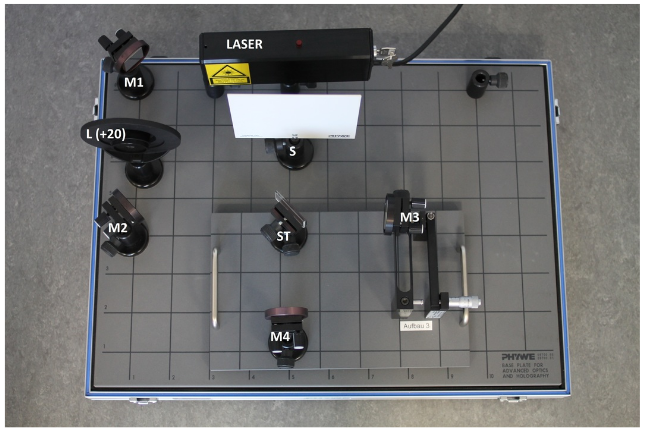
\includegraphics[width=0.7\textwidth]{Aufbau.png}
	\caption{Versuchsaufbau (Quelle: Praktikumsskript)}
	\label{Aufbau}
\end{figure}


\subsection{Versuchsdurchführung}
Mit dem Feinsteinstelltrieb an Spiegel M3 kann die optische Wegl"ange des zugeh"origen Strahlengangs variiert werden, sodass sich das Interferenzmuster am Schirm ver"andert: Pro Verschiebung des Spiegels um eine halbe Wellenl"ange entsteht ein neuer Interferenzring im Zentrum des Musters, das bei weiterer Verschiebung nach au\ss en wandert. Bei umgekehrter Drehrichtung der Mikrometerschraube verschwinden die Interferenzringe im Zentrum. Wir nehmen den Zusammenhang zwischen der optischen Weglänge $d$ und dem Skalenwert $s$ der Mikrometerschraube als linear an und bestimmen in diesem Versuch den Proportionalit"atsfaktor $k$:
\begin{equation}\label{eq:d=ks}
\Delta d=k\cdot \Delta s
\end{equation}
Zu diesem Zweck zählen wir die Anzahl an verschwindenden Interferenzringen $\Delta m$ in Abhängigkeit der Position der Mikrometerschraube $s$.
Wir beginnen bei einem Intensit"atsmaximum im Interferenzzentrum bei $s=7.50mm$, und z"ahlen durch Drehen der Mikrometerschraube 240 Ringe ab, wobei alle 10 Ringe der dazugeh"ohrige Skalenwert der Mikrometerschraube $s$ notiert wird. Die Mikrometerschraube hat eine minimale Skalenbreite von $10\mu m$.

\subsection{Versuchsauswertung}
Unsere Rohdaten sind in Tabelle \ref{table:RohdatenKalibrierung} gelistet.
\begin{table}[H]
	\centering
	\begin{tabular}{|c|c|}
		\hline
		$\Delta m$&$s$ [mm]\\
		0&7.50\\
		10&7.45\\
		20&7.63\\
		30&7.69\\
		40&7.76\\
		50&7.83\\
		60&7.89\\
		70&7.95\\
		80&8.02\\
		90&8.08\\
		100&8.15\\
		110&8.22\\
		120&8.30\\
		130&8.36\\
		140&8.44\\
		150&8.50\\
		160&8.57\\
		170&8.64\\
		180&8.70\\
		190&8.77\\
		200&8.84\\
		210&8.91\\
		220&8.98\\
		230&9.04\\
		240&9.11\\
		\hline
	\end{tabular}
	\caption{Rohdaten Kalibrierung Feinsteinstelltrieb}
	\label{table:RohdatenKalibrierung}
\end{table}
Gl.~\eqref{eq:d=ks} und Gl.~\eqref{eq:Grundgleichung} ergeben den Zusammenhang
\begin{equation}
\Delta m = \frac{2k}{\lambda}\Delta s,
\end{equation}
sodass wir k mit einer linearen Regression bestimmen können. Wir tragen $\Delta m$ gegen $s$ auf und sch"atzen unsere Unsicherheiten folgendermaßen ab:
\begin{align}\label{eq:Unsicherheit_Kalibrierung}
\sigma_{\Delta m}=\frac{1}{\sqrt{12}}\\
\sigma_s=\frac{10\mu m}{\sqrt{12}}
\end{align}
Wir nehmen an, dass wir das Interferenzmaximum gleichverteilt innerhalb der beiden Interferenzminima bei $m+\frac{1}{2}$ und $m-\frac{1}{2}$ bestimmen können. Der Fehler auf $s$ ergibt sich durch den Skalenfehler der minimalen Skalenbreite von $10\mu m$. Die Ergebnisse der Linearen Regression werden in Abb.~\ref{kLinReg} gezeigt.
\begin{figure}[H]
	\centering
	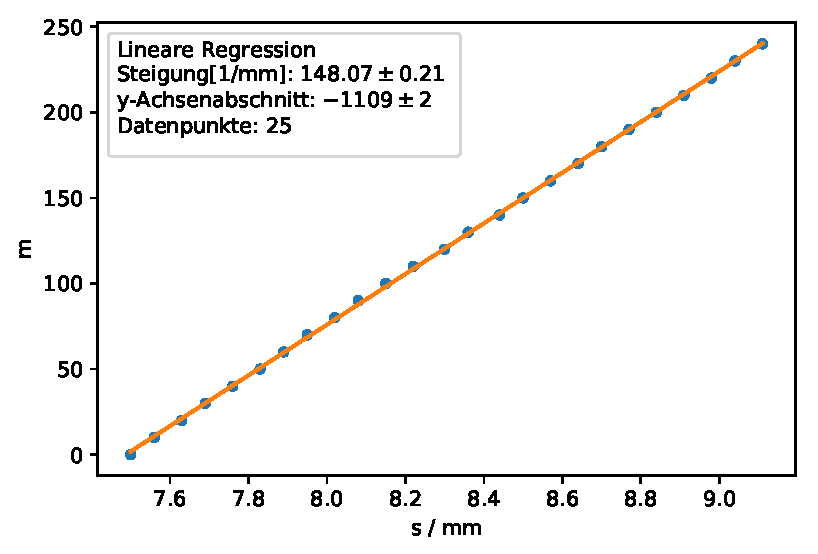
\includegraphics[width=0.6\linewidth]{Python/Uebersetzungsfaktor_LinReg.pdf}
	\caption{Lineare Regression zur Bestimmung des Kalibrierungsfaktors des Feinsteinstelltriebs: Alle Messwerte}
	\label{kLinReg}
\end{figure}
\begin{figure}[H]
	\centering
	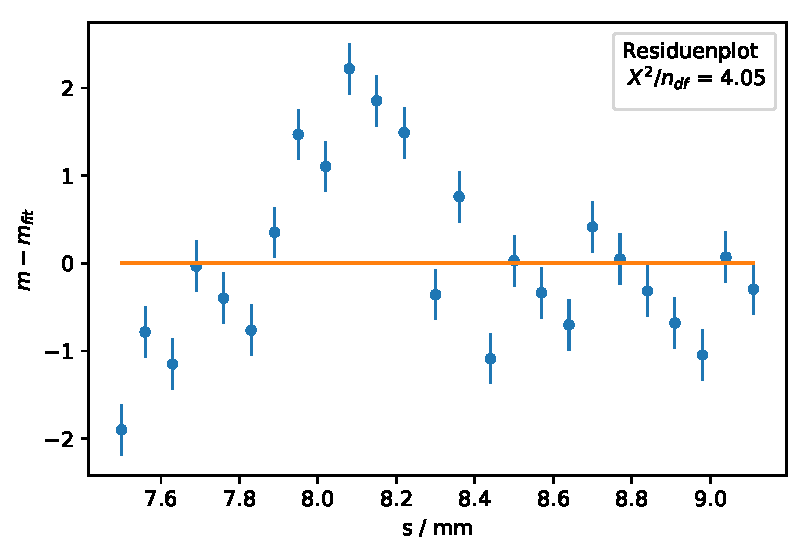
\includegraphics[width=0.6\linewidth]{Python/Uebersetzungsfaktor_Residuen.pdf}
	\caption{Residuenplot zur Bestimmung des Kalibrierungsfaktors des Feinsteinstelltriebs: Alle Messwerte}
	\label{kResPlot}
\end{figure}
Im Residuenplot (Abb.~\ref{kResPlot}) sieht man mehrere Punkte, die um mehr als $\Delta m=1$ von der Ausgleichsgeraden abweichen, was darauf hindeutet, dass wir uns bei der Messung mehrmals verz"ahlt haben. Da  ein Messfehler bewirkt, dass sich auch alle folgenden Messungen um $1\Delta m$ verschieben, sind solche Fehler gerade bei langen Messreihen problematisch. Das $\chi^2/n_{df}$ ergibt folglich einen recht großen Wert von 4.05. Es ist schwierig, im Nachhinein die Position mehrerer Messfehler abzuschätzen, zumal auch nicht direkt ersichtlich ist, ob man sich häufiger um $+\Delta m$ oder um $-\Delta m$ verzählt hat. Daher entscheiden wir uns, die Messreihe in 4 Bereiche einzuteilen und jeweils "uber jeden Teilbereich eine lineare Regression durchzuf"uhren. Die Ergebnisse sind in Abb.~\ref{k1LinReg} und \ref{k1ResPlot} abgebildet f"ur den ersten Messwertebereich, die "ubrigen sind im Anhang zu finden.
\begin{figure}[H]
	\centering
	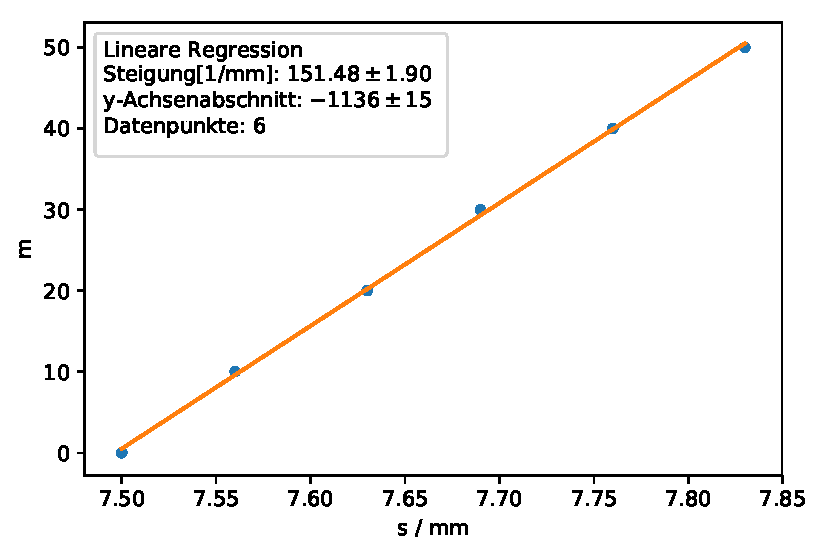
\includegraphics[width=0.6\linewidth]{Python/Uebersetzungsfaktor1_LinReg.pdf}
	\caption{Lineare Regression mit erstem Messwertbereich}
	\label{k1LinReg}
\end{figure}
\begin{figure}[H]
	\centering
	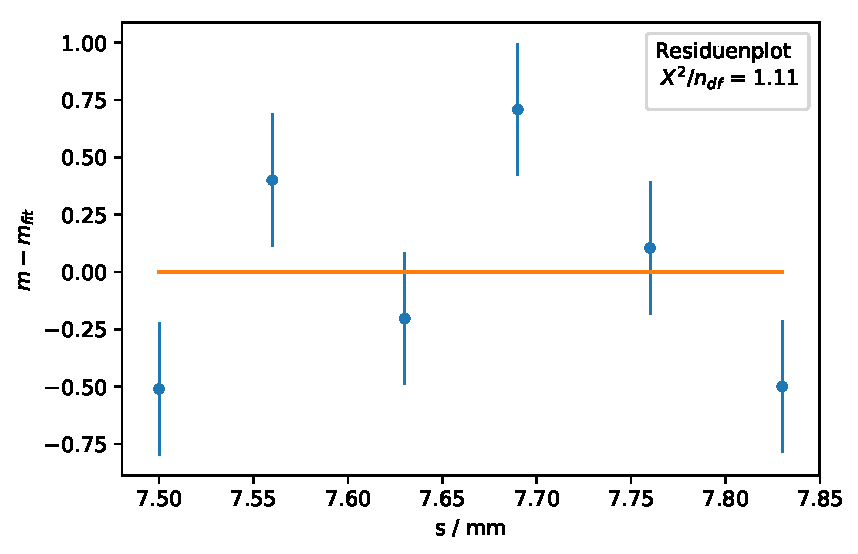
\includegraphics[width=0.6\linewidth]{Python/Uebersetzungsfaktor1_Residuen.pdf}
	\caption{Residuenplot mit erstem Messwertbereich}
	\label{k1ResPlot}
\end{figure}
Die $\chi^2/n$ liegen im Bereich 0.88 bis 1.68, was daf"ur spricht, dass die Ausgleichgerade die Messpunkte gut repr"asentiert, wobei das $\chi^2/n_{df}$ bei der kleinen Anzahl an Messwerten gr"o\ss eren Schwankungen unterliegt. F"ur die vier Messwertbereiche ergeben sich folgende Steigungen $a$
\begin{center}
\begin{tabular}[H]{|c|c|}
	\hline
	&$a$ [1/mm]\\
	\hline
	Messwertreihe 1&$151.48\pm1.90$\\
	Messwertreihe 2&$151.48\pm1.90$\\
	Messwertreihe 3&$146.40\pm1.79$\\
	Messwertreihe 4&$146.58\pm1.42$\\
	\hline
\end{tabular}
\end{center}
Dass zweimal genau die gleiche Steigung berechnet wird, ist aufgrund der geringen Anzahl an Datenpunkten und der groben Skalierung von $s$ mit $10\mu m$ nicht unwahrscheinlich. Da die Steigungen $a$ innerhalb ihrer $1\sigma$-Umgebungen nicht kompatibel sind, berechnen wir den ungewichteten Mittelwert und die Standardabweichung auf den Mittelwert zu
\begin{align}
\overline{a}=148.99\frac{1}{mm}\\
\sigma_{\overline{a}}=\frac{\sigma_{a}}{\sqrt{4}}=1.44\frac{1}{mm}
\end{align}
Aus der Steigung  $a$ l"asst sich der Kalibrierungsfaktor $k$ berechnen "uber 
\begin{equation}
k=\overline{a}\frac{\lambda}{2}.
\end{equation}
Der statistische Fehler auf k pflanzt sich fort aus $\sigma_k(\text{stat})=\frac{\lambda}{2}\sigma_{\overline{a}}$, der systematische Fehler ergibt aus $\sigma_{\lambda}$ mit $\sigma_k(\text{sys})=\sigma_{\lambda}\frac{\overline{a}}{2}$. Insgesamt bekommen wir f"ur den Kalibrierungsfaktor $k$ somit
\begin{equation}
k=0.047139\pm0.000456(\text{stat.})\pm0.000007(\text{sys.}).
\end{equation}


\section{Bestimmung der Wellenlänge}
\subsection{Versuchsaufbau und Durchführung}
In diesem Versuch soll die Wellenlänge eines grünen Lasers mithilfe der eben bestimmten Kalibrierungskonstante $k$ des Feinsteinstelltriebs bestimmt werden. Dazu wird das Lasergerät des roten Lasers gegen das des grünen Lasers ausgetauscht. Sowohl der Versuchsaufbau als auch die Durchführung sind identisch zum vorherigen Versuch. Es werden 270 Maxima durchlaufen im kalibrierten Bereich der Mikrometerschraube $s\in[7.50mm,9.00mm]$.
\subsection{Versuchsauswertung}
\subsubsection{Rohdaten}
\begin{table}[H]\centering
	\begin{tabular}{c||c}
		$\Delta m$&s in mm\\
		\hline
		0&7.5\\
		10&7.55\\
		20&7.61\\
		30&7.66\\
		40&7.71\\
		50&7.77\\
		60&7.82\\
		70&7.88\\
		80&7.94\\
		90&8.00\\
		100&8.05\\
		110&8.11\\
		120&8.16\\
		130&8.21\\
		140&8.28\\
		150&8.34\\
		160&8.39\\
		170&8.45\\
		180&8.51\\
		190&8.56\\
		200&8.62\\
		210&8.67\\
		220&8.73\\
		230&8.79\\
		240&8.85\\
		250&8.90\\
		260&8.96\\
		270&9.01\\
		
	\end{tabular}
	\caption{Rohdaten für s}\label{Tabelle}
\end{table}
\subsubsection{Transformation der Rohdaten und Analyse}
Der Zusammenhang zwischen $\Delta m$ und $s$ ist wie im vorherigen Versuch:
\begin{equation}
2k\Delta s=\lambda m
\end{equation}
Es wird nun $2sk$ gegen $\Delta m$ aufgetragen. Dabei nehmen wir die gleichen Fehler auf $s$ und $\Delta m$ an wie bei der Kalibrierung des Feinsteinstelltriebs (Gl.~\eqref{eq:Unsicherheit_Kalibrierung}). Der Fehler auf $s$ pflanzt sich statistisch auf $2ks$ fort:
\begin{equation}
\sigma_{2ks}=2k\sigma_s
\end{equation}
Die Ergebnisse der linearen Regression werden in Abb.~\ref{Wellenlaenge_LinReg} dargestellt.
\begin{figure}[H]
	\centering
	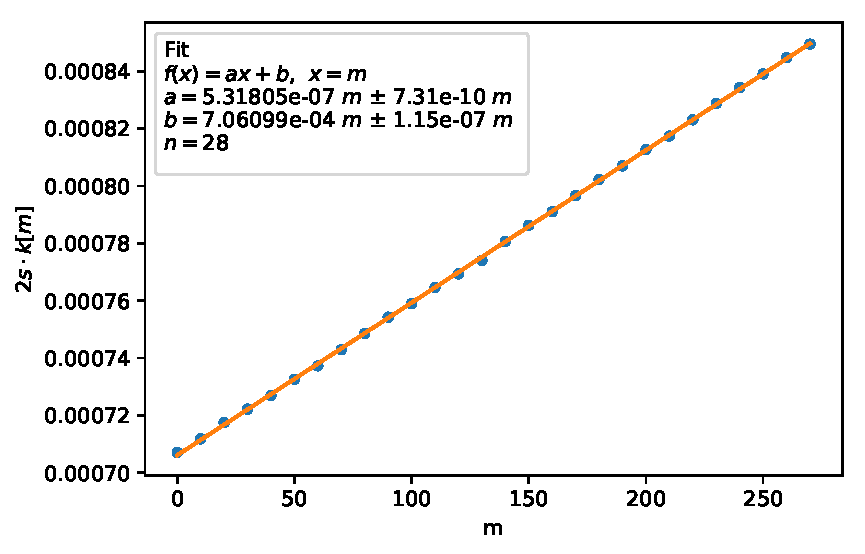
\includegraphics[width=0.6\textwidth]{Python/Lambdagruen_LinReg.pdf}
	\caption{Lineare Regression zur Bestimmung der Wellenlänge}
	\label{Wellenlaenge_LinReg}
\end{figure}
\begin{figure}[H]
	\centering
	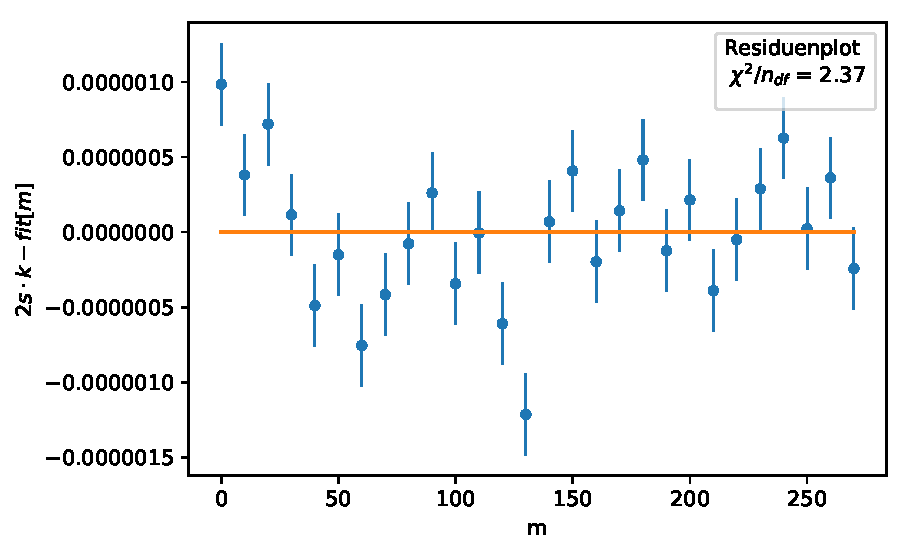
\includegraphics[width=0.6\textwidth]{Python/Lambdagruen_Residuen.pdf}
	\caption{Residuenplot}
\end{figure}
Wir erhalten die Wellenl"ange direkt aus der Steigung zu $\lambda=(531.81\pm0.73)nm$. Das $\chi^2/n_{df}$ ist mit 2.37 zu hoch - ein Hinweis darauf, dass beim Abzählen Fehler gemacht wurden. 
Der Fehler auf $k$ pflanzt sich hier als systematischer Fehler auf $\lambda$ fort. Zur Bestimmung von $\sigma_{\lambda}(sys.)$ nutzen wir die Verschiebemethode und führen zwei weitere lineare Regressionen durch, einmal mit $k\rightarrow k+\sigma_k$ und einmal mit $k\rightarrow k-\sigma_k$. Graphisch ist die Verschiebemethode in diesem Fall dadurch gekennzeichnet, dass, wie der Name impliziert, alle Messpunkte um einen konstanten Wert nach oben bzw. unten verschoben werden. Da sich aber auch der Fehler auf $2k\Delta s$ verändert, erhalten wir unterschiedliche Steigungen und damit Wellenlängen bei der linearen Regression.
\begin{figure}[H]
	\centering
	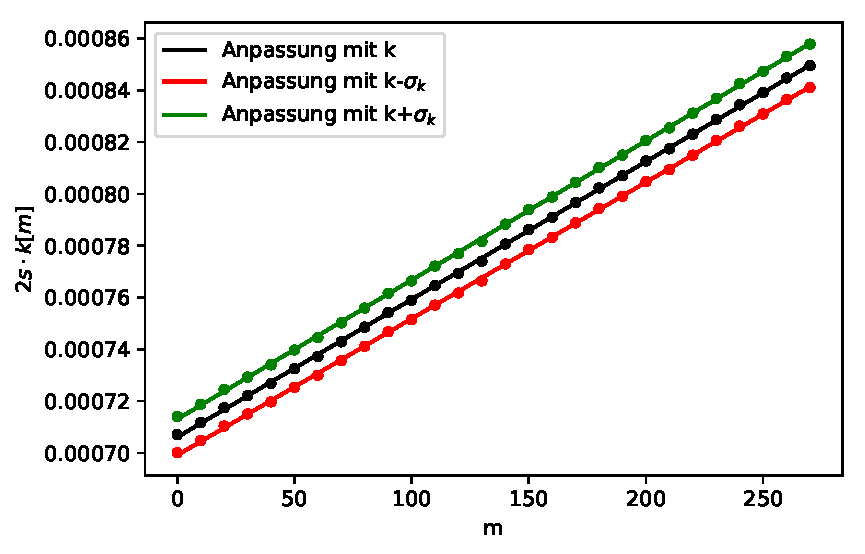
\includegraphics[width=0.6\textwidth]{Python/Lambdagruen_LinReg4.pdf}
	\caption{Veschiebemethode zur Bestimmung der systematischen Unsicherheit auf $\lambda$}
\end{figure}
Für $k\rightarrow k+\sigma_k$ erhalten wir eine Wellenlänge von $\lambda_+=537.038nm$, für $k\rightarrow k-\sigma_k$ erhalten wir eine Wellenlänge von $\lambda_-=526.571nm$. Weitere Ergebnisse und Residuenplots der linearen Regressionen finden sich im Anhang. Wir wählen als systematische Unsicherheit die größere Differenz der verschobenen Wellenlängen zur berechneten Wellenlänge:
\begin{equation}
\sigma_{\lambda}(sys.)=\max\{(\lambda_+-\lambda),(\lambda-\lambda_-)\}=5.234nm
\end{equation}
Die Auswertung ergibt somit eine Wellenlänge von:
\begin{align*}
\lambda = (531.81 \pm 0.73(stat.) \pm 5.23(sys.)) nm
\end{align*}
Das Resultat für die Wellenlänge liegt im $1\sigma$ Bereich der Herstellerangabe von $\lambda=532nm$.

\section{Druckabhängigkeit des Brechungsindexes von Luft}
\subsection{Versuchsaufbau und Durchführung}
Als nächstes wird die Druckabhängigkeit des Brechungsindexes von Luft untersucht. Dazu wird in den Strahlengang zwischen Strahlteiler und Spiegel M4 eine Glasparzelle (hohler Glaszylinder) der Länge $L=10mm$ befestigt. Die Glasparzelle ist über zwei Schläuche an einem digitalen Druckmessgerät und an einer Handpumpe angeschlossen. Über die Handpumpe kann der Druck in der Parzelle verringert werden, wobei der konkrete Wert des Luftdrucks am Messgerät auf 1hPa genau ausgelesen werden kann. Zunächst wird bei Normaldruck, in unserem Fall 995hPa, durch Drehen der Mikrometerschraube ein Interferenzbild erzeugt mit einem Maximum im Zentrum. Nun wird langsam der Druck in der Glasparzelle erniedrigt und bei jeder Entstehung eines neuen Interferenzrings im Zentrum der Druck notiert. Wir beenden einen Messvorgang, wenn wir einen Druck von ca. 300hPa erreichen. Insgesamt wurden 8 Messreihen durchgeführt.

\subsection{Auswertung}
Die Rohdaten der 8 Messreihen sind in Tabelle \ref{table:RohdatenDruck} aufgelistet.
\begin{table}[H]
	\centering
	\begin{tabular}{|c|c|c|c|c|c|c|c|c|}
		\hline
		&\multicolumn{8}{c|}{Druck $P$ der Messreihen (MR) in hPa}\\
		$\Delta m$&MR 0&MR 1&MR 2&MR 3&MR 4&MR 5&MR 6&MR 7\\
		\hline
		0&995&995&995&995&995&995&995&995\\
		1&869&930&850&902&880&900&896&904\\
		2&804&842&761&772&786&811&807&822\\
		3&718&725&659&700&642&719&712&708\\
		4&613&645&557&600&496&618&614&625\\
		5&508&539&450&490&392&520&504&513\\
		6&410&420&360&390&312&413&459&420\\
		7&312&316&270&300&&375&390&302\\
		8&220&&&&&278&353&\\
		9&&&&&&&325&\\
		10&&&&&&&260&\\
		\hline
	\end{tabular}
	\caption{Rohdaten Druckabh"angigkeit Brechungsindex}
	\label{table:RohdatenDruck}
\end{table}
Wir messen eine Leckrate von $0.23hPa/s$ und $0.17hPa/s$. Da die Werte für den Druck immer sofort ausgelesen wurden und wir die Unsicherheit auf den Druck als deutlich größer als die Leckrate annehmen, wird die Leckrate im folgenden vernachlässigt. Der vom Wetterdienst angegebene Außendruck betrug an dem Tag 994hPa, der gemessene Außendruck 999hPa und der Normaldruck in der Glasparzelle 995hPa. Diese Werte decken sich im Rahmen der später angenommenen bzw. berechneten Unsicherheiten. Ein Druck-Offset im Druckmessgerät ist für unsere Berechnungen irrelevant, solange die Druckvdifferenzen richtig gemessen werden.\\
\\
Wir werten diese Daten auf zwei unterschiedliche Arten aus.\\
\\
\textbf{Methode 1}\\
\\
Bei dieser Methode werden die Messreihen zunächst einzeln ausgewertet.\\
Der optische Weg verändert sich mit Gl.~\eqref{eq:d=nl} zu $\Delta d=2L\cdot\Delta n$. Eingesetzt in $d=m\lambda$ als Bedingung für konstruktive Interferenz ergibt sich:
\begin{align}
2L\Delta n&=\lambda\Delta m\nonumber\\
\Leftrightarrow\Delta m&=\frac{\Delta n}{\Delta P}\frac{2L}{\lambda}\Delta P
\end{align}
Gesucht ist der Faktor $\frac{\Delta n}{\Delta P}$, um die Druckabhängigkeit des Brechungsindexes in linearer Näherung $n(P)=1+\frac{\Delta n}{\Delta P}\cdot P$ angeben zu können.\\
Im Folgenden schreiben wir $m=\Delta m$ und meinen die Anzahl an Interferenzringen, die wir ausgehen vom Normaldruck z"ahlen konnten.\\
Wir tragen für jede Messreihe $m$ gegen $P$ auf und führen eine lineare Regression durch. Dabei nehmen wir folgenden Unsicherheiten an:
\begin{align}
\sigma_{m}&=0.1\\
\sigma_{P}&=5hPa
\end{align}
Für den Wert von $\sigma_m$ nehmen an, dass wir die Zahl der Interferenzringe richtig abzählen, aber die genaue Position des Interferenzmaximums nicht exakt bestimmen können. Insbesondere war das Muster sehr sensitiv auf Bewegungen des Schlauchsystems. Die Unsicherheit auf $P$ ist recht groß gewählt, weil sich mit der Handpumpe der Druck nur grob einstellen lies. Es passierte häufiger, dass man zu viel Luft auf einmal rauspumpte und das Interferenzmaximum nicht traf, sodass der Wert für den Druck geschätzt wurde.\\
Die Ergebnisse der linearen Regression sind beispielhaft anhand der Messreihe 6 in Abb.~\ref{MR6_Rohdaten} dargestellt.
\begin{figure}[H]
	\centering
	\begin{subfigure}{0.49\textwidth}
		\centering
		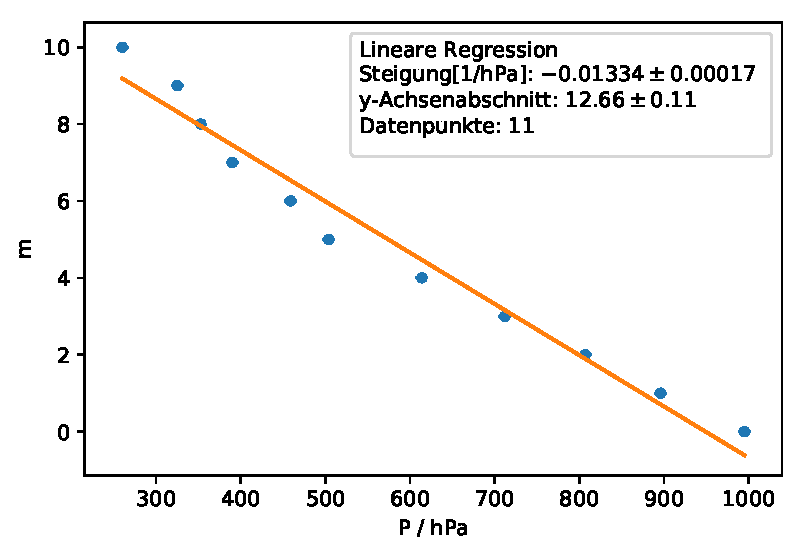
\includegraphics[width=\textwidth]{Python/MR6_LinReg_Rohdaten.pdf}
	\end{subfigure}
	\begin{subfigure}{0.49\textwidth}
		\centering
		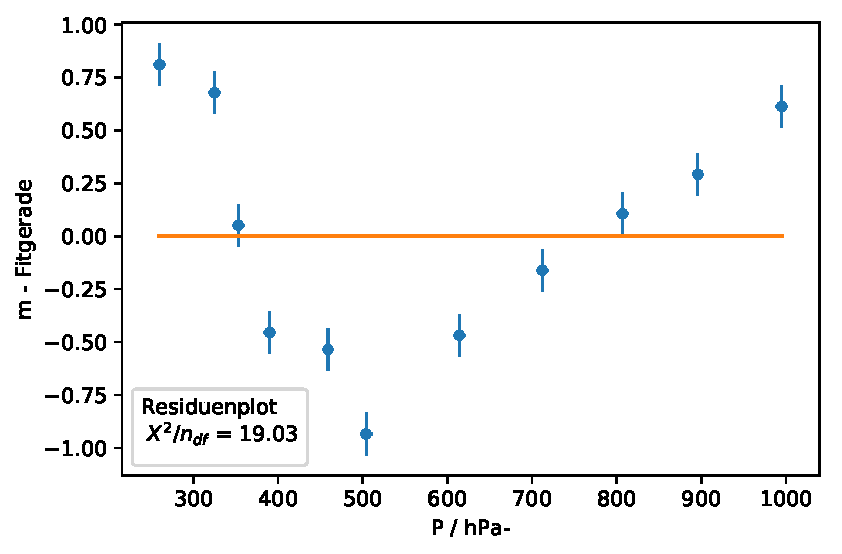
\includegraphics[width=\textwidth]{Python/MR6_Residuen_Rohdaten.pdf}
	\end{subfigure}
	\caption{Lineare Regression mit den Rohdaten der Messreihe 6}
	\label{MR6_Rohdaten}
\end{figure}
Im Residuenplot ist zu erkennnen, dass die letzten 5 Messpunkte nicht mit der linearen Struktur der vorherigen Datenpunkte übereinstimmen. Wir vermuten, dass wir einen Fehler beim Abzählen gemacht haben oder sich durch Stöße das Interferenzbild verändert hat. Für Veränderungen im Interferenzbild spricht auch, dass wir das Interferenzmaximum bei Normaldruck häufig nach einer Messreihe neu einstellen mussten, weil es leicht verschoben war. Daher lassen wir die letzten fünf Punkte in MR 6 weg und aus analogen Gründen auch den ersten Punkt bei MR 2 und die letzten beiden Punkte aus MR 5. Im Anhang finden sich die zugehörigen Graphen der linearen Regression.\\
Wir führen mit den korrigierten Messreihen erneut eine lineare Regression durch. In Messreihe 6 sieht man beispielhaft, dass die Ausgleichsgerade die Punkte nun besser beschreibt. Das $\chi^2/n_{df}$ ist mit 0.34 aber nun etwas zu klein.
\begin{figure}[H]
	\centering
	\begin{subfigure}{0.49\textwidth}
		\centering
		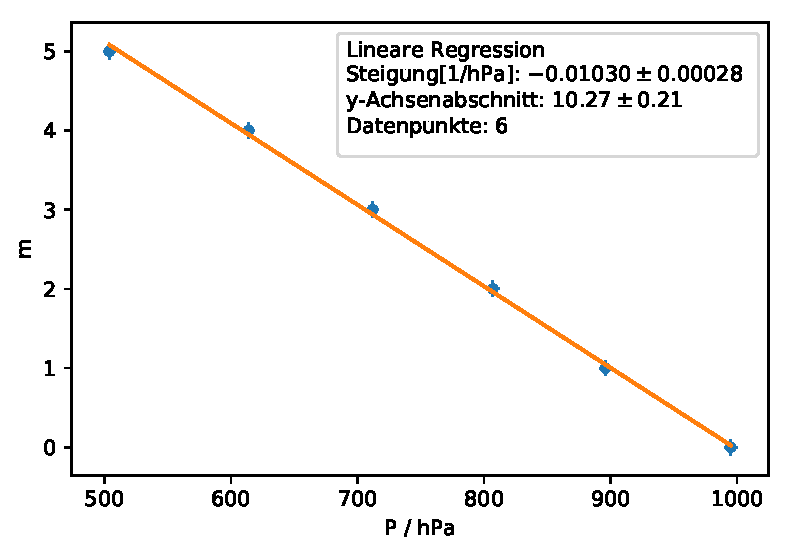
\includegraphics[width=\textwidth]{Python/MR6_LinReg.pdf}
	\end{subfigure}
	\begin{subfigure}{0.49\textwidth}
		\centering
		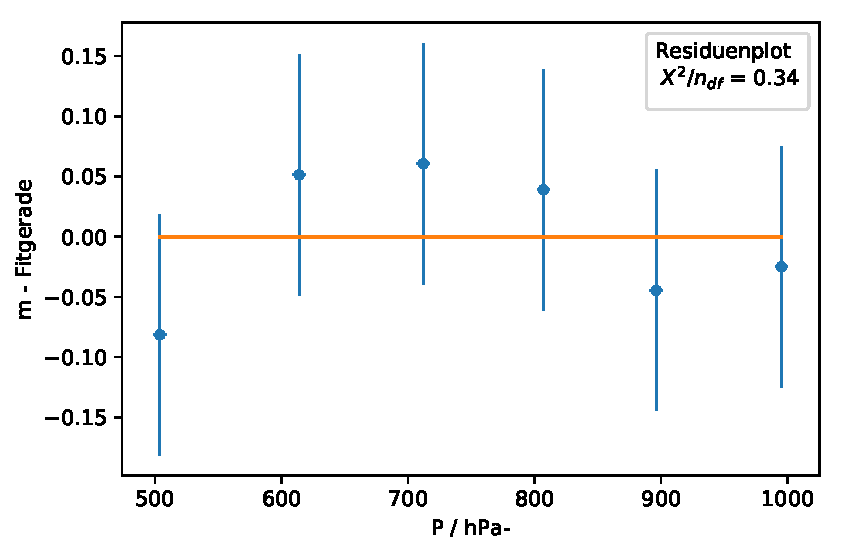
\includegraphics[width=\textwidth]{Python/MR6_Residuen.pdf}
	\end{subfigure}
	\caption{Lineare Regression mit den korrigierten Daten der Messreihe 6}
	\label{MR6_LinReg}
\end{figure}
Die Werte für $\chi^2/n_{df}$  der anderen Messreihen befinden sich im Bereich von 0.33 bis 2.68 (MR 4), was heißt, dass es große Diskrepanzen zwischen den Messreihen gibt. Aus den Steigungen $a$ lassen sich nun $\frac{\Delta n}{\Delta P}$ mit Unsicherheit $\sigma$ pro Messreihe bestimmen, durch
\begin{align}\label{eq:dndp_aus_Steigung}
\frac{\Delta n}{\Delta P}&=a\frac{\lambda}{2L}\nonumber\\
\sigma(stat)&=\sigma_{a}\frac{\lambda}{2L}\nonumber\\
\sigma(sys)&=\sigma_{\lambda}\frac{a}{2L}
\end{align}
Die Ergebnisse sind in Tabelle \ref{table:Methode1_dndP} zusammengefasst und in Abb.~\eqref{Methode1_dndP} grafisch aufbereitet.
\begin{table}[H]
	\centering
	\begin{tabular}{|c|c|c|c|c|}
		\hline
		Messreihe&Steigung a [$10^{-2}$/hPa]&$\Delta n/\Delta P$ [$10^{-7}$/hPa]&$\sigma_{\text{stat}}$[$10^{-7}$/hPa]&$\sigma_{\text{sys}}$[$10^{-7}$/hPa]\\
		\hline
		0&1.038$\pm$0.015&2.761&0.040&0.031\\
		1&1.009$\pm$0.017&2.684&0.046&0.030\\
		2&1.017$\pm$0.022&2.705&0.057&0.030\\
		3&1.002$\pm$0.017&2.665&0.046&0.030\\
		4&0.841$\pm$0.017&2.235&0.046&0.025\\
		5&1.037$\pm$0.022&2.757&0.059&0.031\\
		6&1.030$\pm$0.028&2.738&0.074&0.031\\
		7&1.013$\pm$0.018&2.693&0.047&0.030\\
		\hline
	\end{tabular}
	\caption{Steigung und resultierendes $\Delta n/\Delta P$ pro Messreihe}
	\label{table:Methode1_dndP}
\end{table}
\begin{figure}[H]
	\centering
	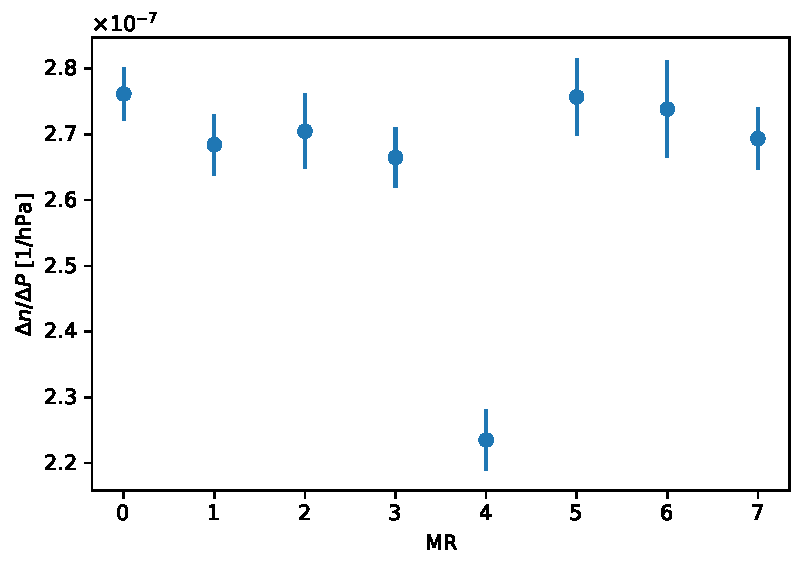
\includegraphics[width=0.6\textwidth]{Python/Methode1_Ergebnisse.pdf}
	\caption{$\Delta n/\Delta P$ für die unterschiedlichen Messreihen mit statistischem Fehler}
	\label{Methode1_dndP}
\end{figure}
Wie in der Abbildung deutlich zu erkennen ist, stellt MR 4 einen Ausreißer dar. Die anderen Werte f"ur $\frac{\Delta n}{\Delta P}$ sind in ihren Unsicherheiten kompatibel. Daher berechnen wir das gewichtete Mittel aus allen Messreihen außer MR 4. In Methode 2 stellen wir fest, dass bei der MR 2 ein Maximum übersprungen wurde, was die große Abweichung zu den anderen MR erklärt. Die systematischen Fehler sind ähnlich groß für alle Messreihen, weshalb wir für das gewichtete Mittel den größeren systematischen Fehler $\sigma(sys)=0.31$ auswählen. Insgesamt erhalten wir als Endergebnis:  
\begin{equation}
\frac{\Delta n}{\Delta P}=(2.713\pm 0.019(\text{stat.})\pm 0.031(\text{sys.}))\cdot10^{-7}\frac{1}{hPa}
\end{equation}
Der Literaturwert von $2.655\cdot10^{-7}\frac{1}{hPa}$ liegt in einer $1.2\sigma$-Umgebung.\\
\\
\textbf{Methode 2}\\
\\
Bei dieser Methode werden zunächst alle Druckwerte für jeden Wert von $m$ gemittelt und dann nur eine lineare Regression mit den Mittelwerten durchgeführt.\\
Wir hatten bereits bei der vorherigen Methode festgestellt, dass bei den letzten 5 Werten von MR 6 und bei den letzten 2 Werten von MR 5 wahrscheinlich Fehler bei der Durchführung des Versuchs gemacht wurden, und lassen diese Werte auch bei dieser Auswertung weg. In Abb.~\ref{Methode2vorKorr} sind die übrigen Messdaten aufgetragen.
\begin{figure}[H]
	\centering
	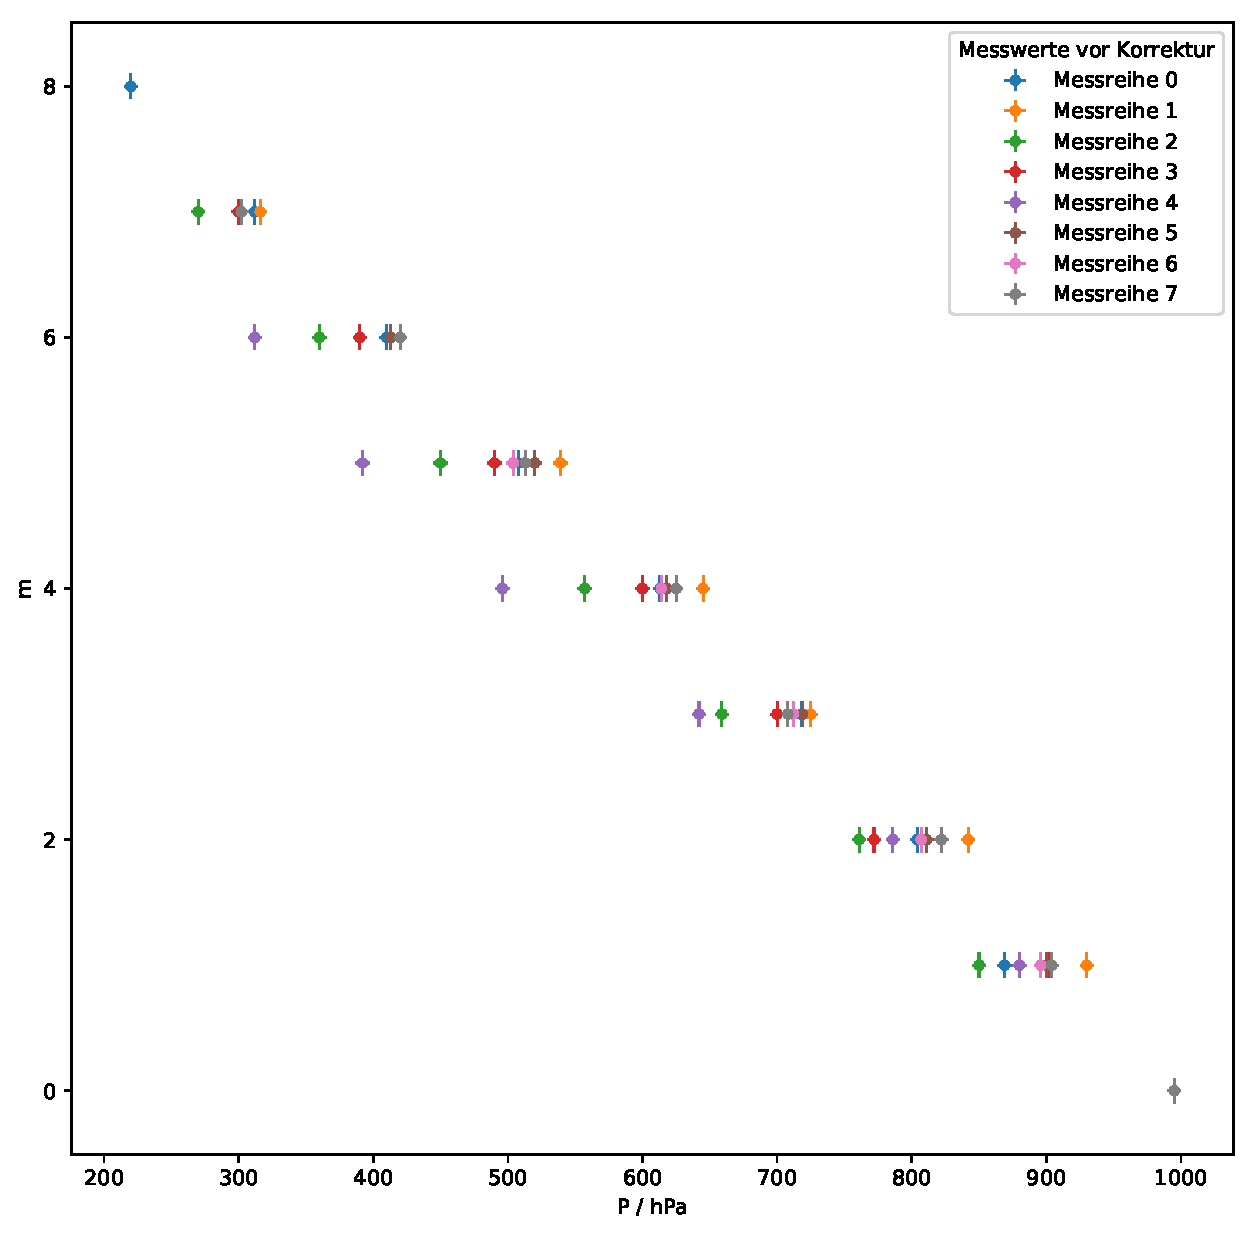
\includegraphics[width=0.7\textwidth]{Python/Methode2vorKorr.pdf}
	\caption{Rohdaten zur Druckabhängigkeit des Brechungsindexes, wobei die letzten 2 Werte aus MR 5 und die letzten 5 Werte aus MR 6 nicht hinzugenommen wurden}
	\label{Methode2vorKorr}
\end{figure}
Man sieht Besonderheiten bei MR 2 (gr"un) und bei MR 4 (violet). MR 2 scheint um einen konstanten Druck in Richtung kleinerer Drücke verschoben zu sein. Vermutlich liegt das daran, dass das Interferenzmuster für $m=0$ nicht richtig eingestellt war. Wir korrigieren diese Verschiebung folgendermaßen: Wir berechnen die Differenz aus dem Mittelwert aller Drücke bei $m=1$ und dem konkreten Druck $P_{MR2,m=1}$  und addieren diese Differenz auf alle Messwerte aus MR 2 (außer dem ersten Messwert).\\
Als nächstes betrachten wir MR 4. Diese war bereits bei der vorherigen Methode 1 aufgefallen, weil ihr Wert für $\frac{\Delta n}{\Delta P}$ nicht mit denen der anderen MR kompatibel war. In Abb.~\ref{Methode2vorKorr} l"asst sich erkennen, dass wir das das Interferenzmaximum mit $m=3$ übersprungen haben müssem. Das heißt, der Druck P=642hPa sollte eigentlich bei $m=4$ eingetragen sein, der Druck P=496hPa bei $m=5$ usw. Wir korrigieren und verschieben die Werte entsprechend. Für m=3 wählen wir den Mittelwert der übrigen Messreihen.\\
Mit diesen Korrekturen sehen unsere Messwerte folgendermaßen aus (Abb.~\ref{Methode2nachKorr}).
\begin{figure}[H]
	\centering
	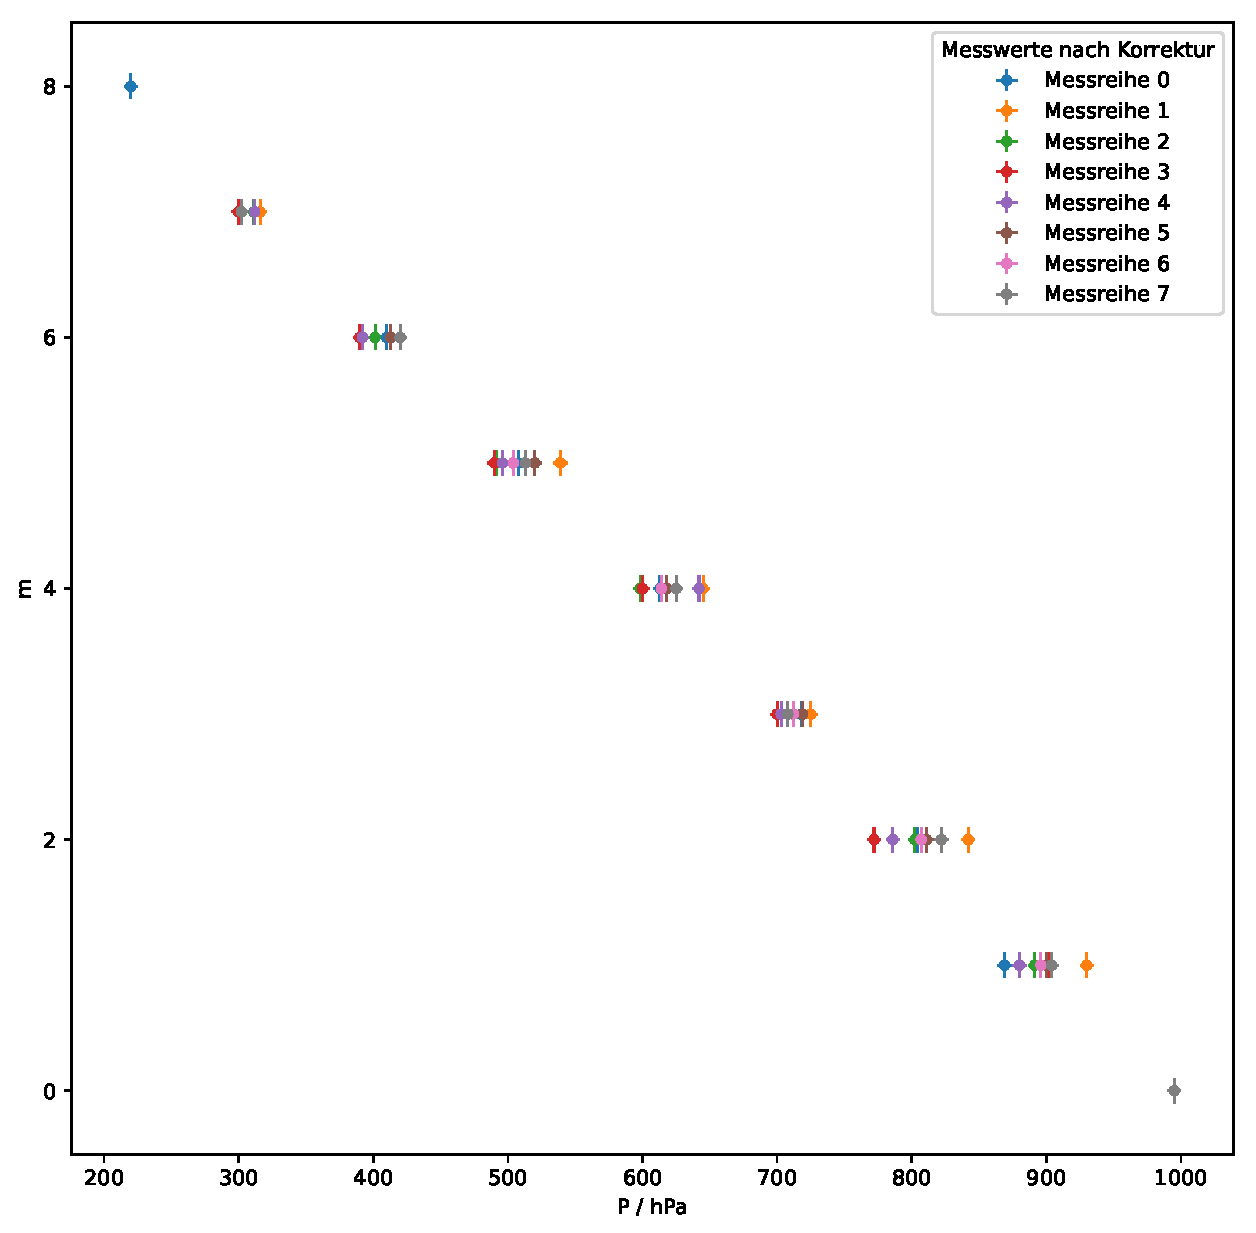
\includegraphics[width=0.7\textwidth]{Python/Methode2nachKorr.pdf}
	\caption{korrigierte Messwerte}
	\label{Methode2nachKorr}
\end{figure}
Wir berechnen nun für jedes $m$ im Bereich $[0,7]$ den Mittelwert der Druckwerte und die Unsicherheit auf den Mittelwert gemäß
\begin{equation}
\sigma_{\overline{P}}=\frac{\sigma_P}{\sqrt{N}}
\end{equation}
Den Fehler auf $P_{m=0}=995$ setzen wir auf den Mittelwert der "ubrigen Unsicherheiten.Die Ergebnisse sind in Tabelle \ref{table:Methode2} gelistet.
\begin{table}[H]
	\centering
	\begin{tabular}{|c|r|r|r|r|r|r|r|r|}
		\hline
		$m$&0&1&2&3&4&5&6&7\\
		\hline
		$\overline{P}$ / hPa&995.0&896.5&805.8&710.7&619.2&507.7&406.6&308.9\\
		$\sigma_{\overline{P}}$ / hPa&4.6&6.4&7.5&3.3&6.1&5.8&4.7&2.3\\
		\hline
	\end{tabular}
	\caption{gemittelte Werte f"ur P}
	\label{table:Methode2}
\end{table}
Nun tragen wir $m$ gegen die gemittelten Drücke auf und führen eine lineare Regression durch, wobei wir wie in Methode 1 $\sigma_m=0.1$ annehmen. Die Ergebnisse werden in Abb.~\ref{gemittelterDruck_LinReg} dargestellt.
\begin{figure}[H]
	\centering	
	\begin{subfigure}{0.49\textwidth}
		\centering
		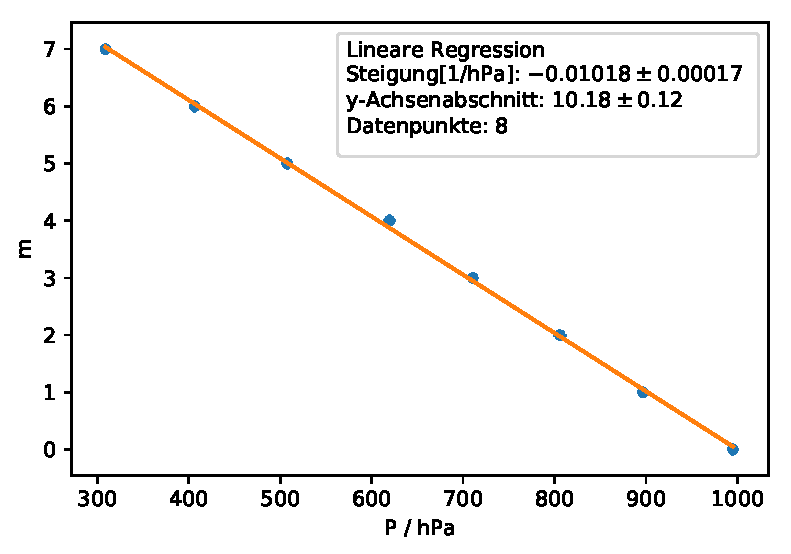
\includegraphics[width=\textwidth]{Python/gemittelterDruck_LinReg.pdf}
	\end{subfigure}
	\begin{subfigure}{0.49\textwidth}
		\centering
		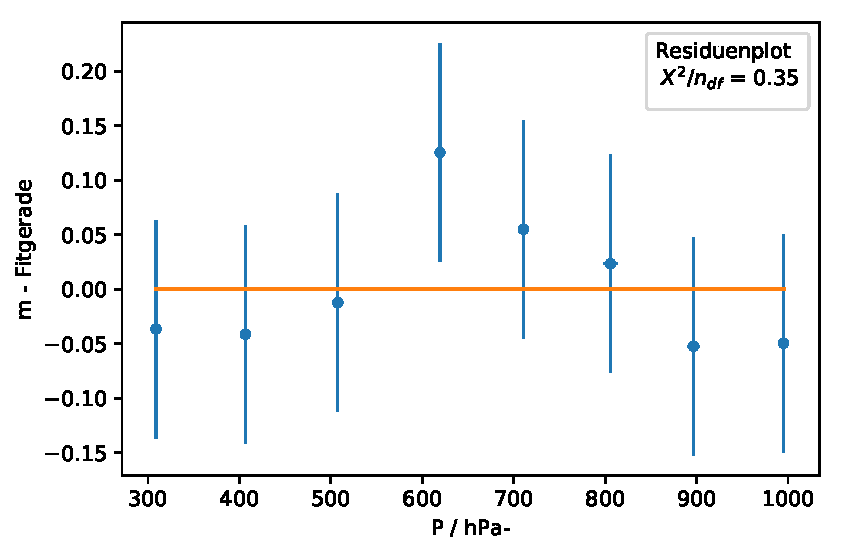
\includegraphics[width=\textwidth]{Python/gemittelterDruck_Residuen.pdf}
	\end{subfigure}
	\caption{Lineare Regression mit gemittelten Drücken}
	\label{gemittelterDruck_LinReg}
\end{figure}
Im Residuenplot ist ein kleiner Sprung bei $m=4$ erkennbar, den wir aber aufgrund der geringen Datenmenge auf statistische Schwankungen zurückführen. Das $\chi^2/n_{df}$ ist mit 0.35 relativ klein, was darauf hindeutet, dass wir die Position der Interferenzringe doch besser bestimmen konnten, als erwartet. Aus der Steigung der linearen Regression l"asst sich analog zu Methode 1 $\frac{\Delta n}{\Delta P}$ bestimmen (Gl.~\eqref{eq:dndp_aus_Steigung}). Das Ergebnis lautet:
\begin{equation}
\frac{\Delta n}{\Delta P}=(2.708\pm 0.046(\text{stat.})\pm 0.030(\text{sys.}))\cdot10^{-7}\frac{1}{hPa}
\end{equation}
Der Literaturwert liegt in einer $1\sigma$-Umgebung. 

\section{Brechungsindex von $\text{CO}_2$}
\subsection{Versuchsaufbau und Durchführung}
In diesem Versuch bestimmen wir den Brechungsindex von CO$_2$. Dazu werden das Druckmessgerät und die Handpumpe von den Schläuchen, die zur Glasparzelle führen, abgenommen und einer der Schläuche mit einer CO$_2$-Gasdruckflasche verbunden. Der andere Schlauch wird mit einer Klemme so gehalten, dass das offene Schlauchende nach oben zeigt. Mithilfe der Mikrometerschraube wird ein Maximum im Interferenzbild eingestellt. Nun wird langsam das Ventil der CO$_2$-Flasche geöffnet, sodass das CO$_2$ in die Glasparzelle eindringt und die darin vorhandene Luft allmählich verdrängt. Man zählt die Anzahl der Ringe $m$, die im Zentrum des Interferenzbildes verschwinden. Nach kurzer Zeit bleibt das Bild stehen: Die Luft in der Glasparzelle wurde vollständig durch CO$_2$ ersetzt, und das CO$_2$ bleibt in der Glasparzelle liegen, weil es schwerer ist als Luft. Man schätzt ab, wie weit oder nah das Bild am vorherigen Interferenzmaximum entfernt ist, sodass $m$ nicht zwingend ganzzahlig ist. Der Versuch wird 3 Mal wiederholt. Das CO$_2$ wird nach jedem Versuch mit der Handpumpe aus der Glasparzelle gepumpt. Zur einfacheren Zählbarkeit auch bei schnellem CO$_2$-Einfluss wird das Interferenzbild mit einer Kamera aufgenommen.


\subsection{Auswertung}
Es konnte nur das erste Video ausgewertet werde, weil bei den anderen Messreihen das CO$_2$ zu schnell in die Glasparzelle eingeströmt ist und die Interferenzringe nicht zählbar waren.\\
Im ersten Video zählen wir $m=5.0$ Interferenzmaxima.\\
Für die Anzahl der Interferenzmaxima und der Änderung des Brechungsindexes gilt folgender Zusammenhang:
\begin{equation}
\Delta n=\frac{\lambda}{2L}\Delta m
\end{equation}
Da wir Luft durch CO$_2$ ersetzt haben, ergibt sich der Brechungindex von CO$_2$ nun zu
\begin{align}
n_{\text{CO}_2}&=n_{\text{Luft}}+\Delta n\nonumber\\
&=1+\frac{\Delta n}{\Delta P}\cdot P+\frac{\lambda}{2L}\Delta m
\end{align}
Wir setzen folgende Werte ein:
\begin{align}
\frac{\Delta n}{\Delta P}&=(2.7078\pm 0.0765)\cdot 10^{-7}\frac{1}{hPa}\\
\lambda&=(531.805\pm 5.965)nm\\
L&=10mm\\
P&=994hPa\pm 1hPa\\
\Delta m&=5.0\pm 0.1\\
\end{align}
Die Werte f"ur $\lambda$ und $\frac{\Delta n}{\Delta P}$ stammen aus den vorherigen Versuchen, wobei f"ur $\frac{\Delta n}{\Delta P}$, das Ergebnis von Methode 2 verwendet wurde. Der Wert f"ur P ist durch den Wetterbericht vorgegeben. Den Fehler sch"atzen wir auf 1hPa ab, weil das der Wert ist, den wir bei Normaldruck innerhalb der Glasparzelle gemessen haben. Die Unsicherheit auf $m$ ergibt sich dadurch, dass wir die Lage des Interferenzmaximums nicht exakt ablesen können. Wir erhalten:
\begin{equation}
n_{\text{CO}_2}=1.0004021
\end{equation} 
Die statistische Unsicherheit ergibt sich nur durch $\sigma_{\Delta m}$ zu
\begin{equation}
\sigma_{\text{CO}_2}(stat.)=\frac{\lambda}{2L}\sigma_{\Delta m}=0.0000027
\end{equation}
Die anderen Unsicherheiten wirken sich systematisch auf $n_{\text{CO}_2}$ aus und wir berechnen sie durch Gaußsche Fehlerfortpflanzung. Da $\frac{\Delta n}{\Delta P}$ und $\lambda$ miteinander korrelieren, ergibt sich
\begin{align}
\sigma_{\text{CO}_2}(sys.)&=\sqrt{\left(\frac{\Delta n}{\Delta P}\sigma_P\right)^2+(P\sigma_{\Delta n/\Delta P})^2+\left(\frac{\Delta m}{2L}\sigma_{\lambda}\right)^2+2P\frac{\Delta m}{2L}\sigma_{\Delta n/\Delta P}\sigma_{\lambda}}\nonumber\\
&=0.0000091
\end{align}
Insgesamt also
\begin{equation}
n_{\text{CO}_2}=1.0004021\pm 0.0000027(stat.)\pm 0.0000091(sys.)
\end{equation}
Die Literatur gibt einen Wert von $n_{\text{CO}_2}=1.000416$ an, was in einer $1.2\sigma$-Umgebung des berechneten Wertes liegt.

\newpage
\section{Anhang}

\textbf{Kalibrierung des Feinsteinstelltriebs}
\begin{figure}[H]
	\centering
	\begin{subfigure}{0.49\textwidth}
		\centering
		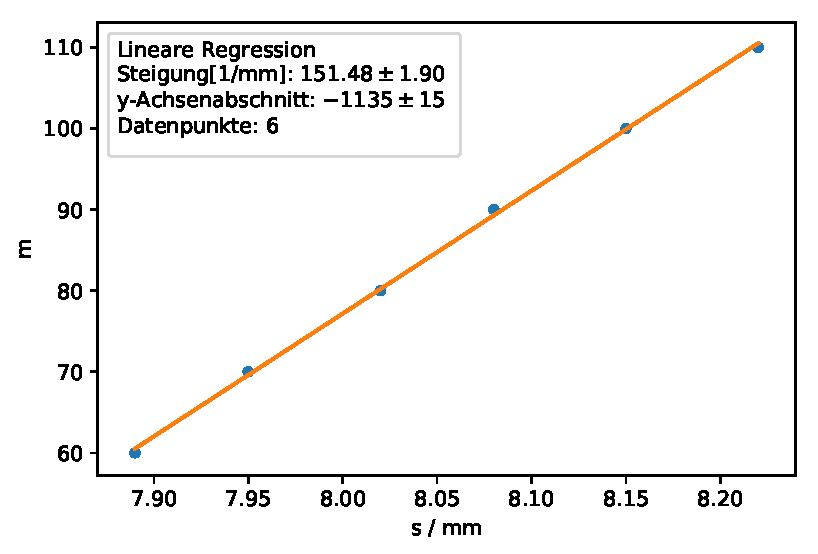
\includegraphics[width=\textwidth]{Python/Uebersetzungsfaktor2_LinReg.pdf}
		\caption{Lineare Regression mit zweitem Messwertbereich}
		\label{k2LinReg}
	\end{subfigure}
	\begin{subfigure}{0.49\textwidth}
		\centering
		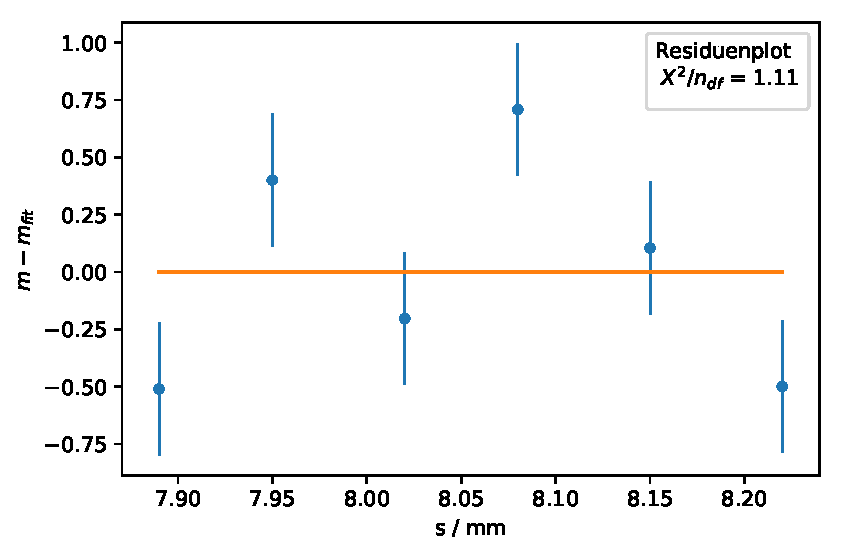
\includegraphics[width=\textwidth]{Python/Uebersetzungsfaktor2_Residuen.pdf}
		\caption{Residuenplot mit zweitem Messwertbereich}
		\label{k2ResPlot}
	\end{subfigure}
	\begin{subfigure}{0.49\textwidth}
		\centering
		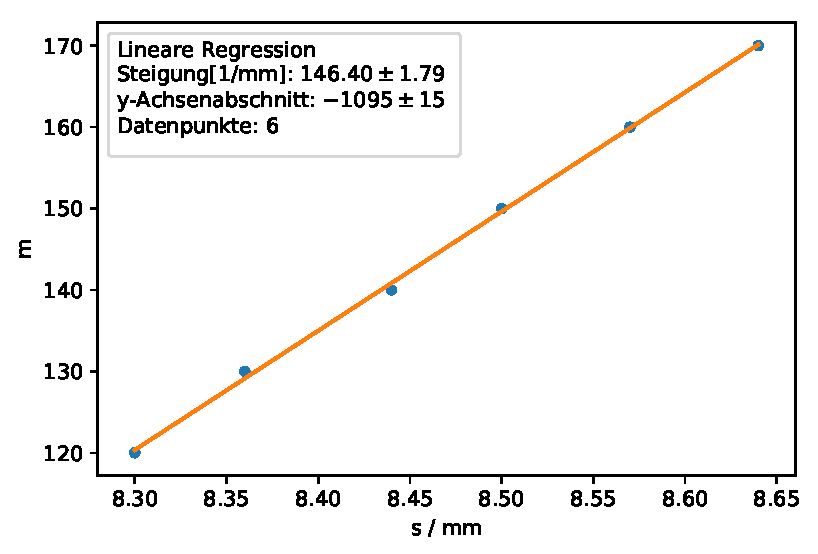
\includegraphics[width=\linewidth]{Python/Uebersetzungsfaktor3_LinReg.pdf}
		\caption{Lineare Regression mit drittem Messwertbereich}
		\label{k3LinReg}
	\end{subfigure}
	\begin{subfigure}{0.49\textwidth}
		\centering
		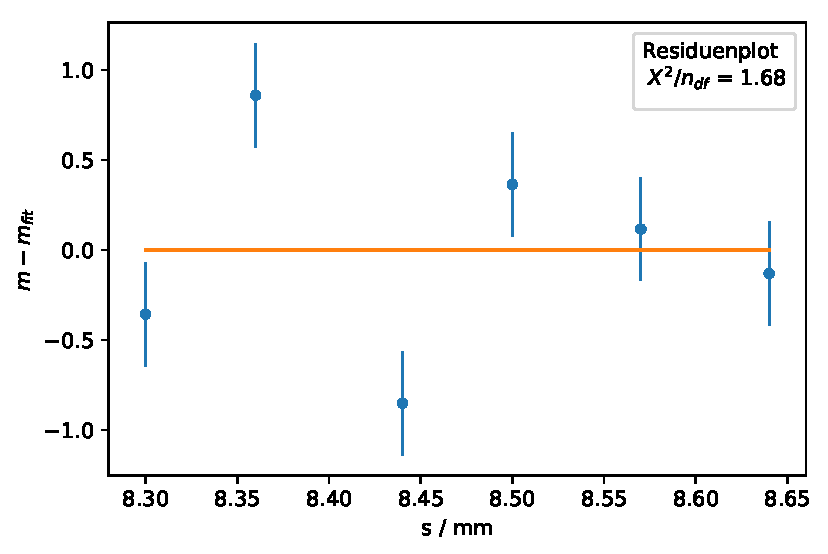
\includegraphics[width=\linewidth]{Python/Uebersetzungsfaktor3_Residuen.pdf}
		\caption{Residuenplot mit drittem Messwertbereich}
		\label{k3ResPlot}
	\end{subfigure}
	\begin{subfigure}{0.49\textwidth}
		\centering
		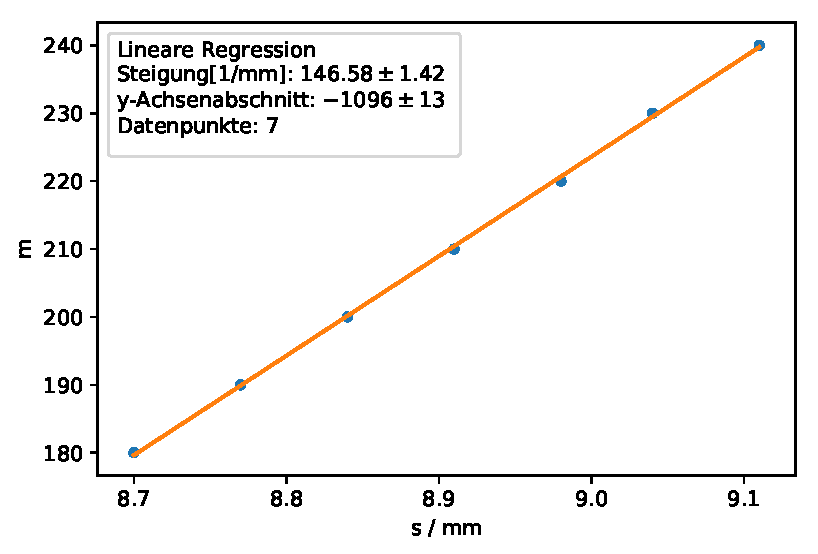
\includegraphics[width=\linewidth]{Python/Uebersetzungsfaktor4_LinReg.pdf}
		\caption{Lineare Regression mit viertem Messwertbereich}
		\label{k4LinReg}
	\end{subfigure}
	\begin{subfigure}{0.49\textwidth}
		\centering
		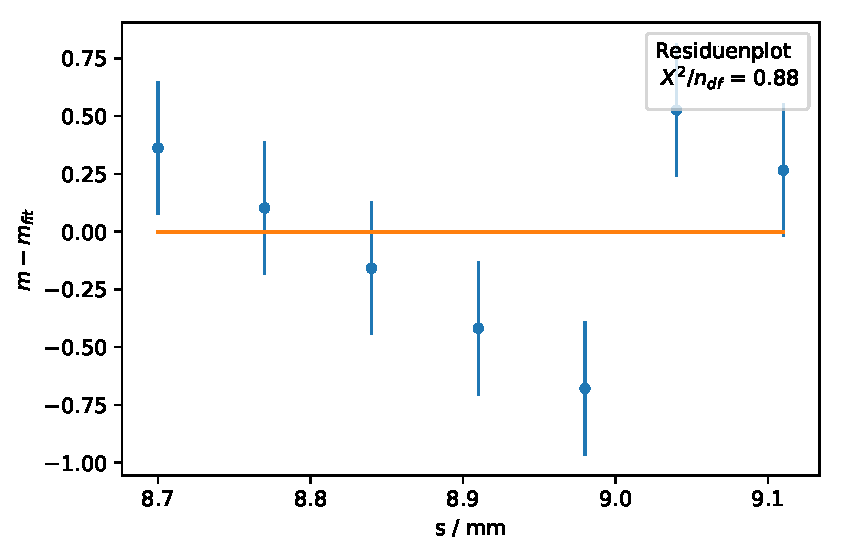
\includegraphics[width=\linewidth]{Python/Uebersetzungsfaktor4_Residuen.pdf}
		\caption{Residuenplot mit viertem Messwertbereich}
		\label{k4ResPlot}
	\end{subfigure}
	\caption{Lineare Regression zur Bestimmung des Kalibrierungsfaktors des Feinsteinstelltriebs}
\end{figure}
\newpage
\textbf{Wellenl"angenbestimmung}
\begin{figure}[H]
	\centering
	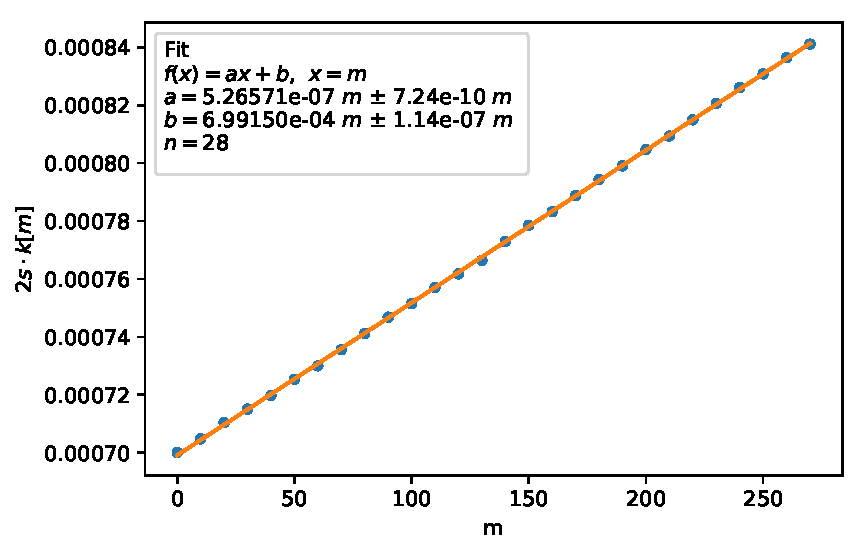
\includegraphics[scale=1.0]{Python/Lambdagruen_LinReg2.pdf}
	\caption{Lineare Regression der Wellenlänge für k-$\sigma_k$}
\end{figure}

\begin{figure}[H]
	\centering
	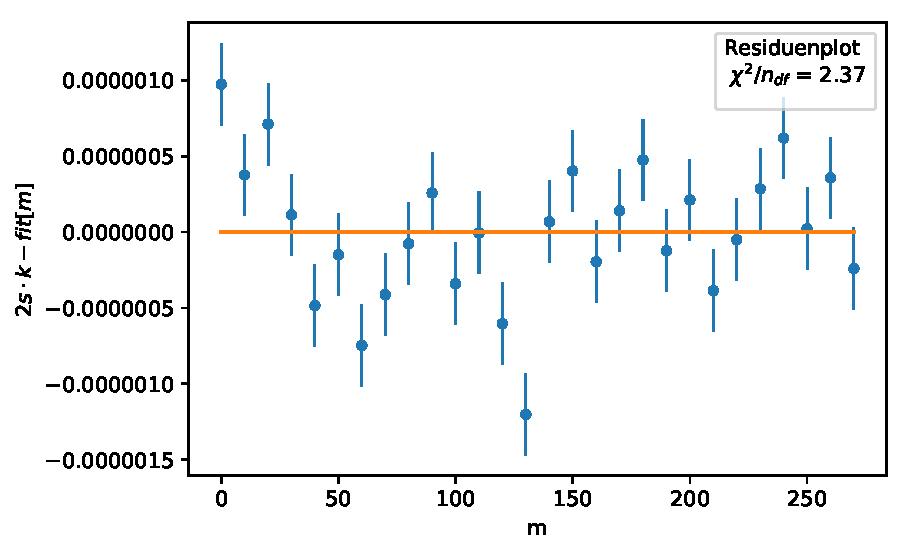
\includegraphics[scale=1.0]{Python/Lambdagruen_Residuen2.pdf}
	\caption{Residuen der Wellenlänge für k-$\sigma_k$}
\end{figure}

\begin{figure}[H]
	\centering
	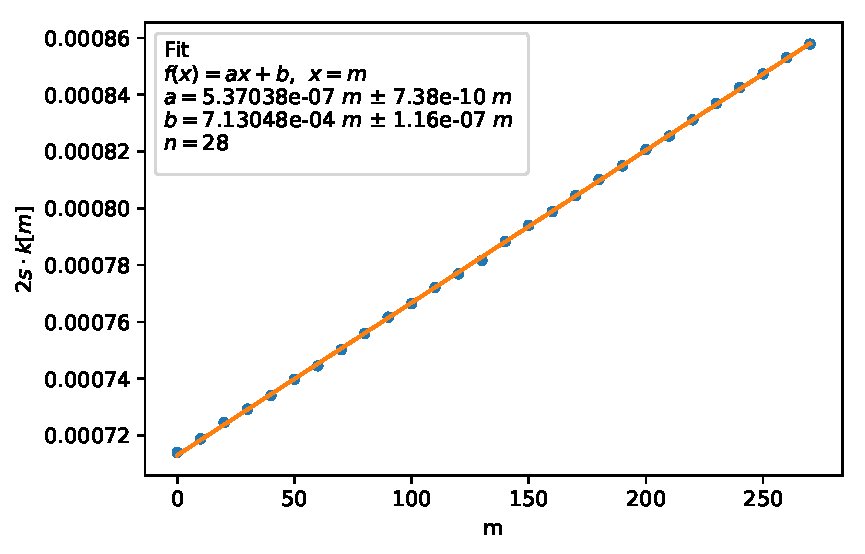
\includegraphics[scale=1.0]{Python/Lambdagruen_LinReg3.pdf}
	\caption{Lineare Regression der Wellenlänge für k+$\sigma_k$}
\end{figure}

\begin{figure}[H]
	\centering
	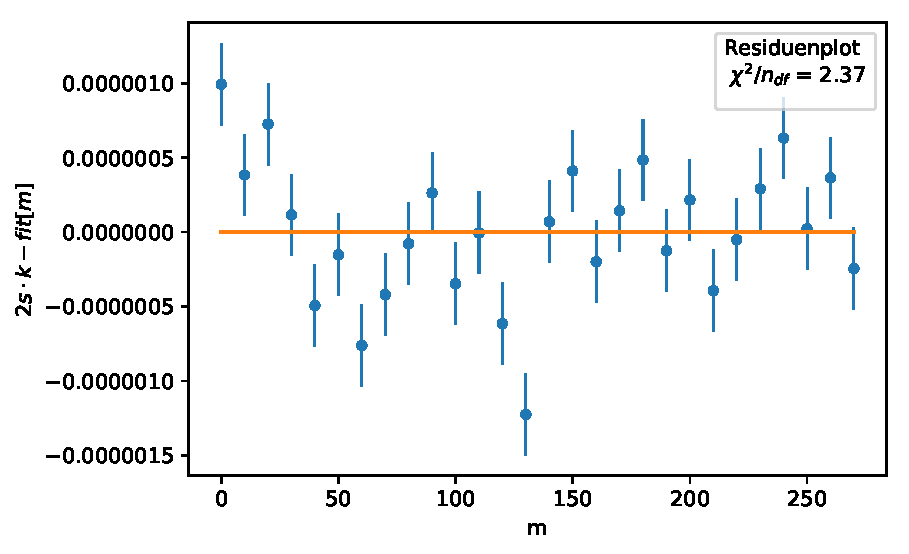
\includegraphics[scale=1.0]{Python/Lambdagruen_Residuen3.pdf}
	\caption{Residuen der Wellenlänge für k+$\sigma_k$}
\end{figure}
\newpage
\textbf{Druckabhängigkeit des Brechungsindexes von Luft}
\begin{figure}[H]
	\centering
	\begin{subfigure}{0.49\textwidth}
		\centering
		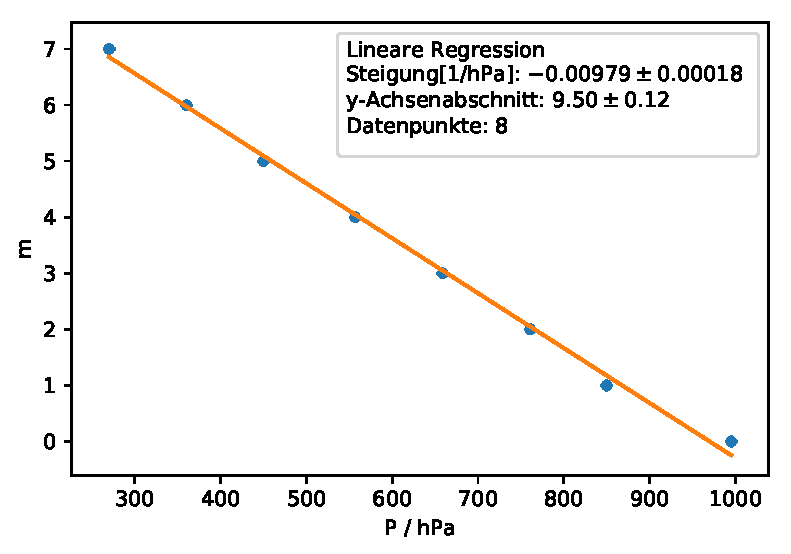
\includegraphics[width=\textwidth]{Python/MR2_LinReg_Rohdaten.pdf}
	\end{subfigure}
	\begin{subfigure}{0.49\textwidth}
		\centering
		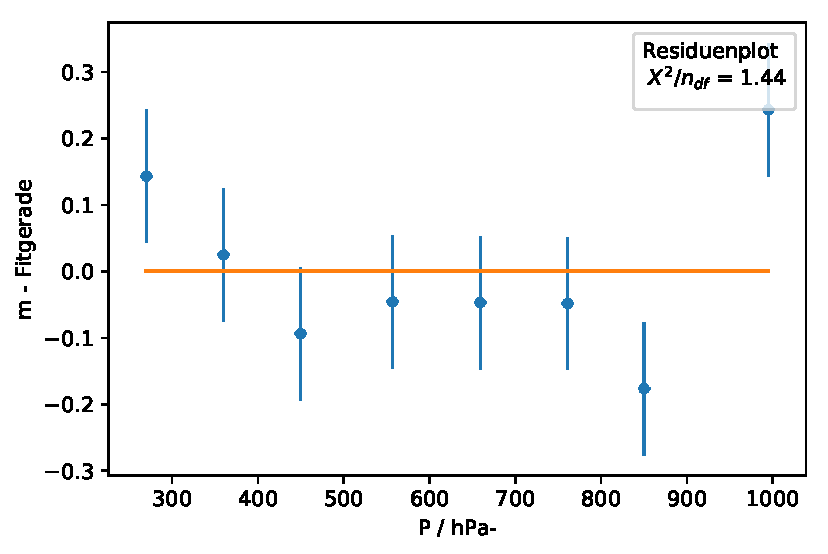
\includegraphics[width=\textwidth]{Python/MR2_Residuen_Rohdaten.pdf}
	\end{subfigure}
	\begin{subfigure}{0.49\textwidth}
		\centering
		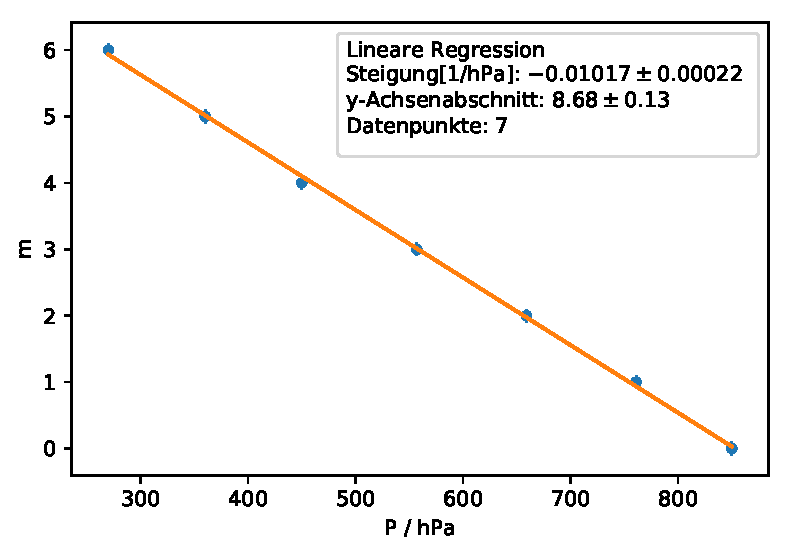
\includegraphics[width=\textwidth]{Python/MR2_LinReg.pdf}
	\end{subfigure}
	\begin{subfigure}{0.49\textwidth}
		\centering
		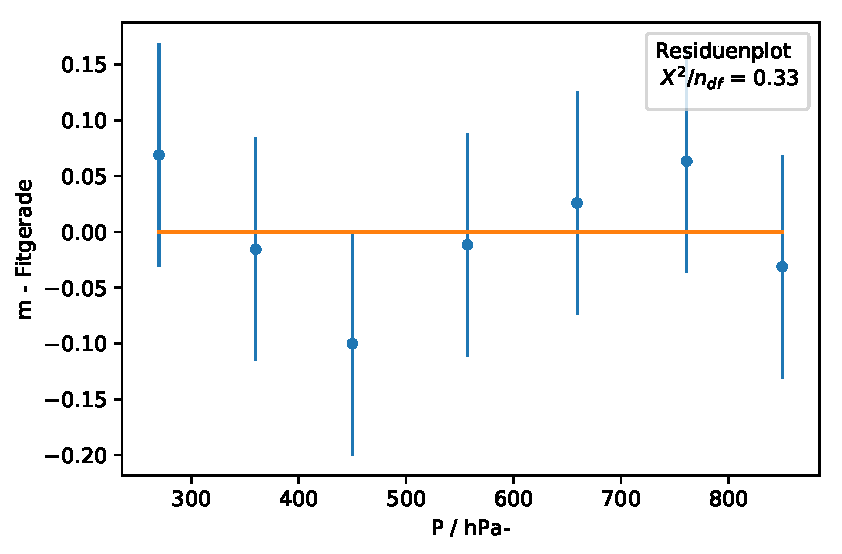
\includegraphics[width=\textwidth]{Python/MR2_Residuen.pdf}
	\end{subfigure}
	\caption{Lineare Regression mit den Rohdaten (oben) und korrigierten Daten (unten) der Messreihe 2}
	\label{MR2_LinReg}
\end{figure}
\begin{figure}[H]
	\centering
	\begin{subfigure}{0.49\textwidth}
		\centering
		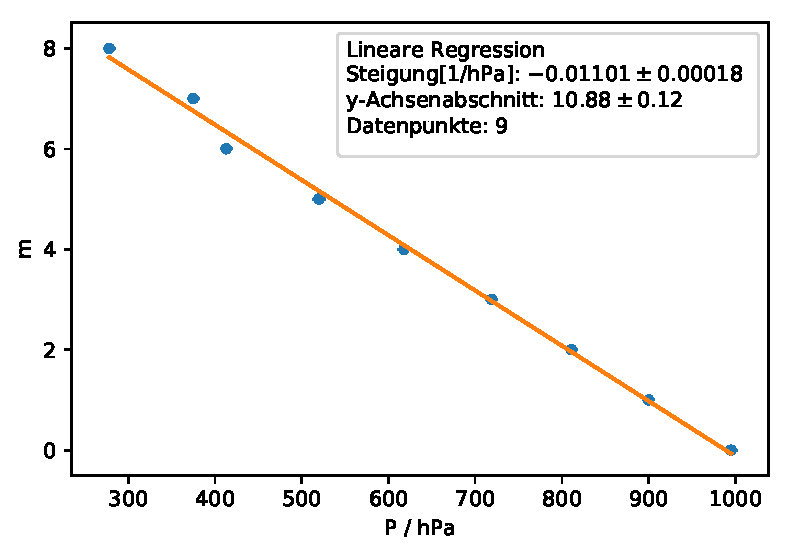
\includegraphics[width=\textwidth]{Python/MR5_LinReg_Rohdaten.pdf}
	\end{subfigure}
	\begin{subfigure}{0.49\textwidth}
		\centering
		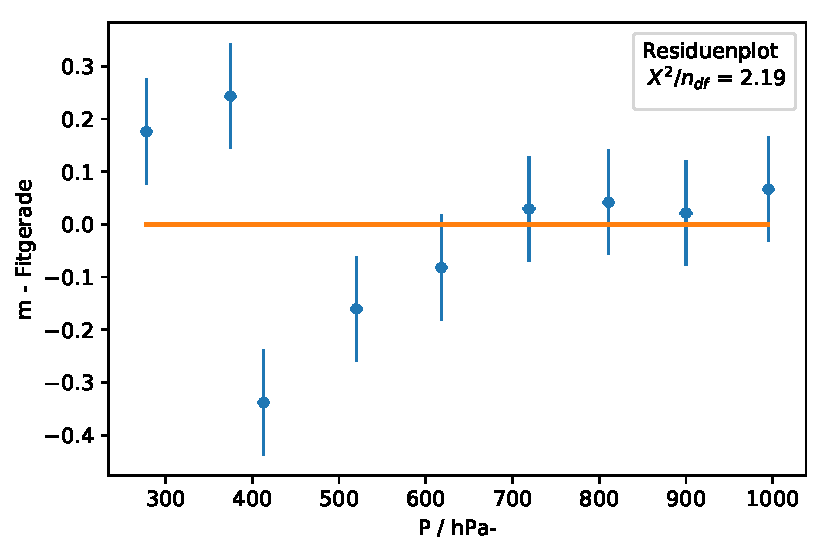
\includegraphics[width=\textwidth]{Python/MR5_Residuen_Rohdaten.pdf}
	\end{subfigure}
	\begin{subfigure}{0.49\textwidth}
		\centering
		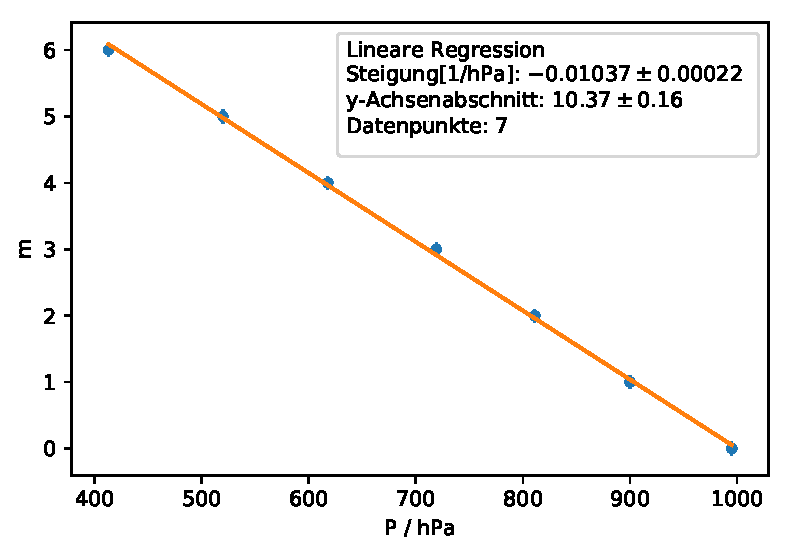
\includegraphics[width=\textwidth]{Python/MR5_LinReg.pdf}
	\end{subfigure}
	\begin{subfigure}{0.49\textwidth}
		\centering
		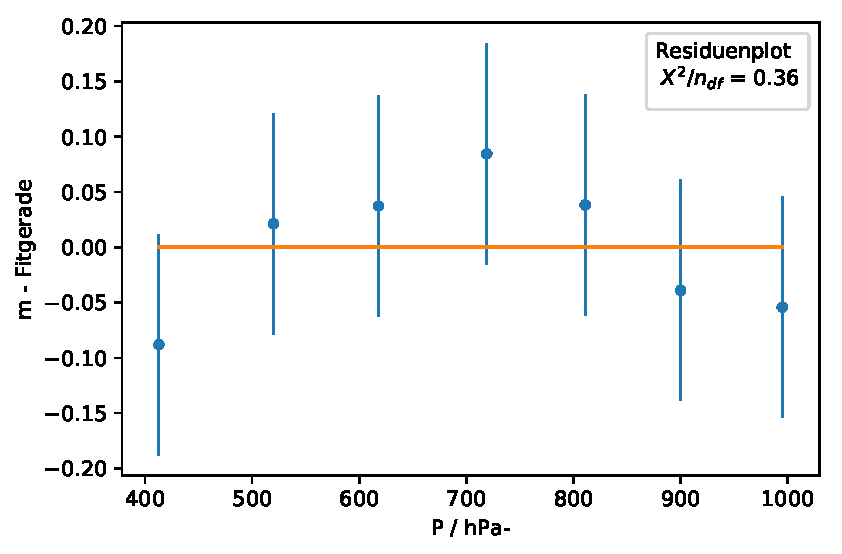
\includegraphics[width=\textwidth]{Python/MR5_Residuen.pdf}
	\end{subfigure}
	\caption{Lineare Regression mit den Rohdaten (oben) und korrigierten Daten (unten) der Messreihe 5}
	\label{MR5_LinReg}
\end{figure}

\begin{figure}[H]
	\centering	
	\begin{subfigure}{0.49\textwidth}
	\centering
	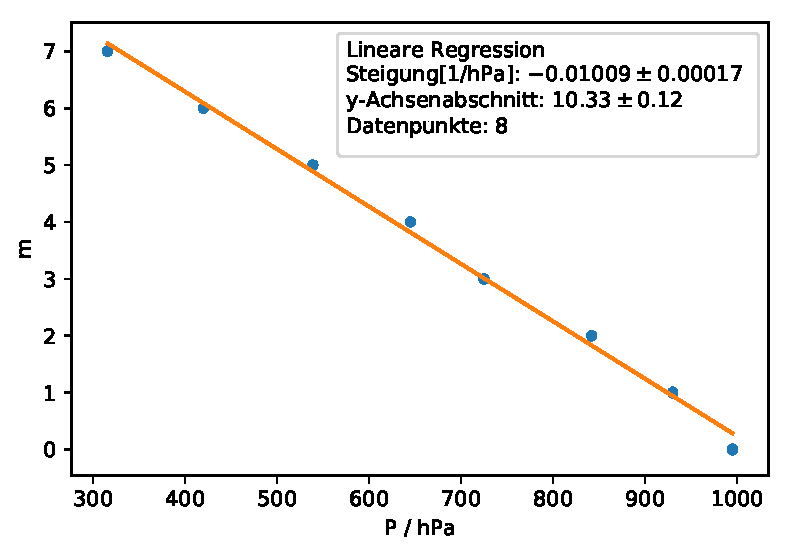
\includegraphics[width=\textwidth]{Python/MR1_LinReg.pdf}
	\end{subfigure}
	\begin{subfigure}{0.49\textwidth}
	\centering
	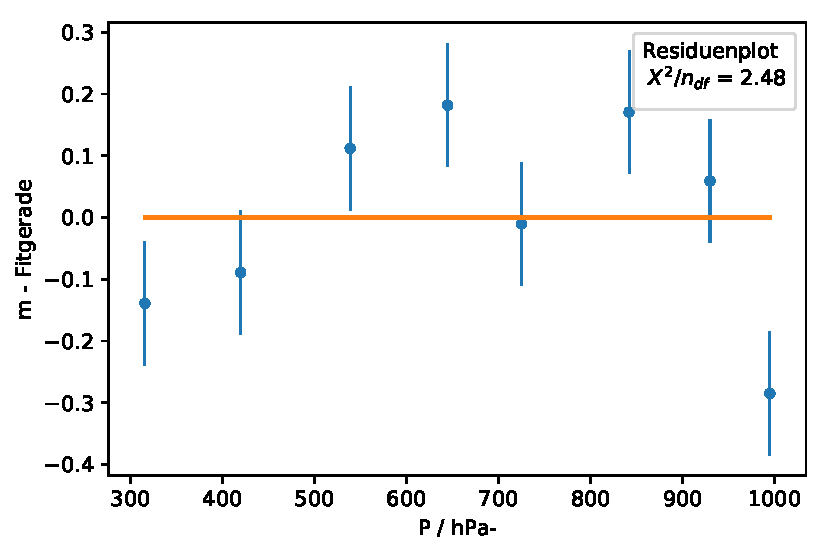
\includegraphics[width=\textwidth]{Python/MR1_Residuen.pdf}
	\end{subfigure}
	\caption{Lineare Regression mit der Messreihe 1}
	\label{MR1_LinReg}
\end{figure}
\begin{figure}[H]
	\centering	
	\begin{subfigure}{0.49\textwidth}
		\centering
		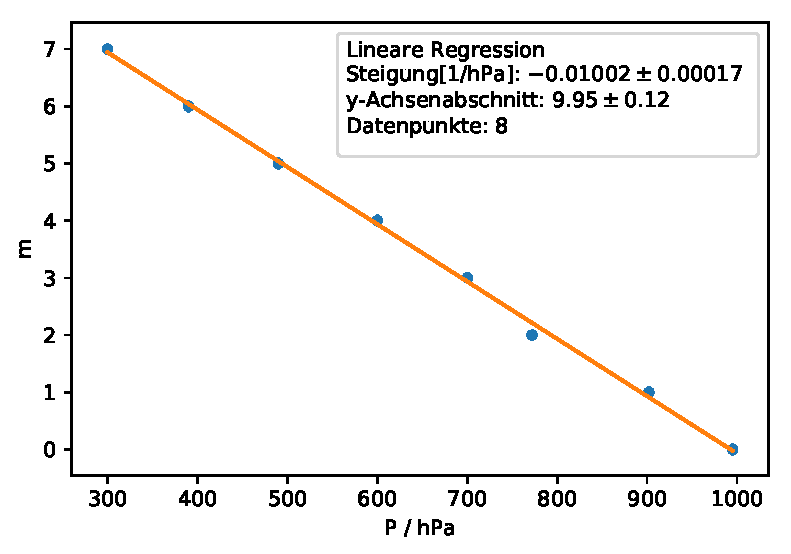
\includegraphics[width=\textwidth]{Python/MR3_LinReg.pdf}
	\end{subfigure}
	\begin{subfigure}{0.49\textwidth}
		\centering
		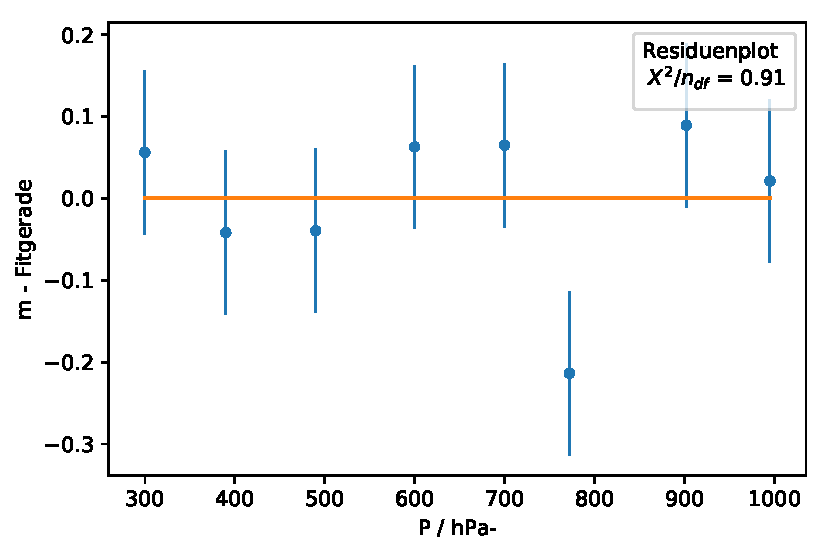
\includegraphics[width=\textwidth]{Python/MR3_Residuen.pdf}
	\end{subfigure}
	\caption{Lineare Regression mit der Messreihe 3}
	\label{MR3_LinReg}
\end{figure}
\begin{figure}[H]
	\centering	
	\begin{subfigure}{0.49\textwidth}
		\centering
		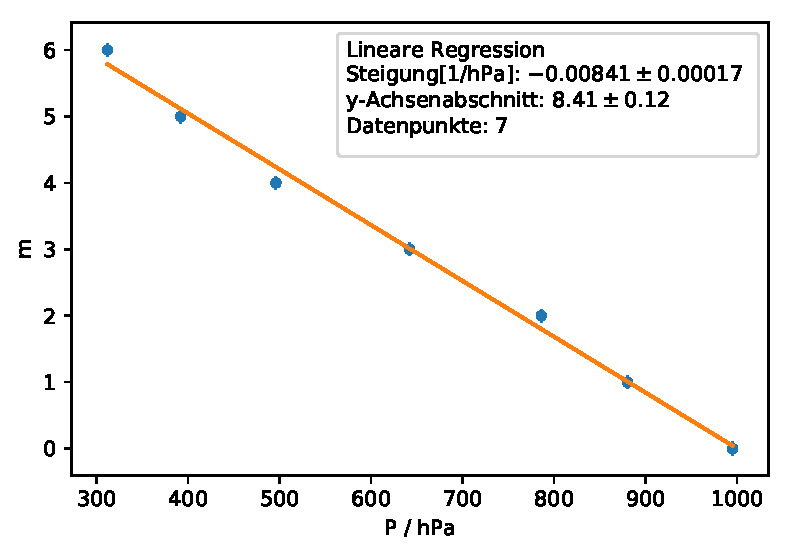
\includegraphics[width=\textwidth]{Python/MR4_LinReg.pdf}
	\end{subfigure}
	\begin{subfigure}{0.49\textwidth}
		\centering
		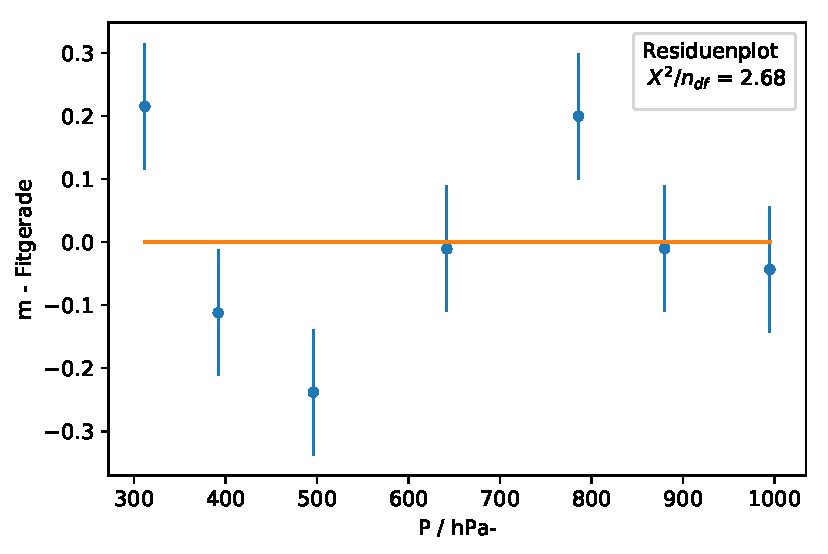
\includegraphics[width=\textwidth]{Python/MR4_Residuen.pdf}
	\end{subfigure}
	\caption{Lineare Regression mit der Messreihe 4}
	\label{MR4_LinReg}
\end{figure}
\begin{figure}[H]
	\centering	
	\begin{subfigure}{0.49\textwidth}
		\centering
		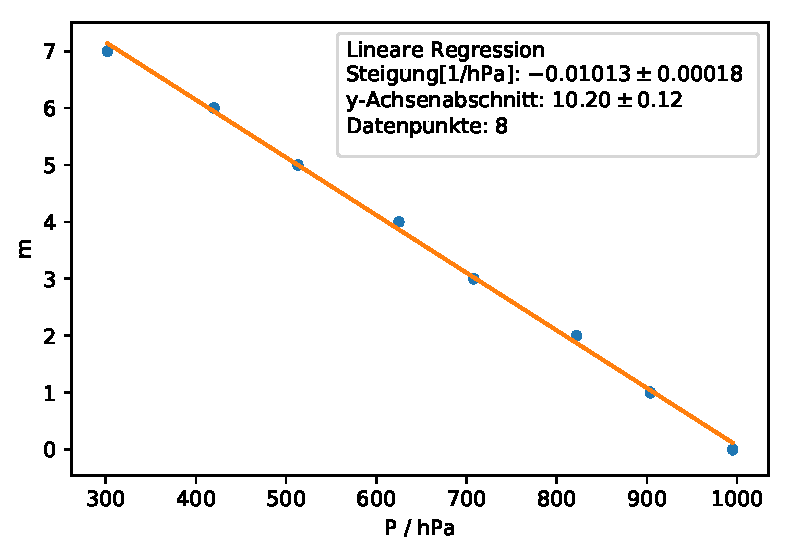
\includegraphics[width=\textwidth]{Python/MR7_LinReg.pdf}
	\end{subfigure}
	\begin{subfigure}{0.49\textwidth}
		\centering
		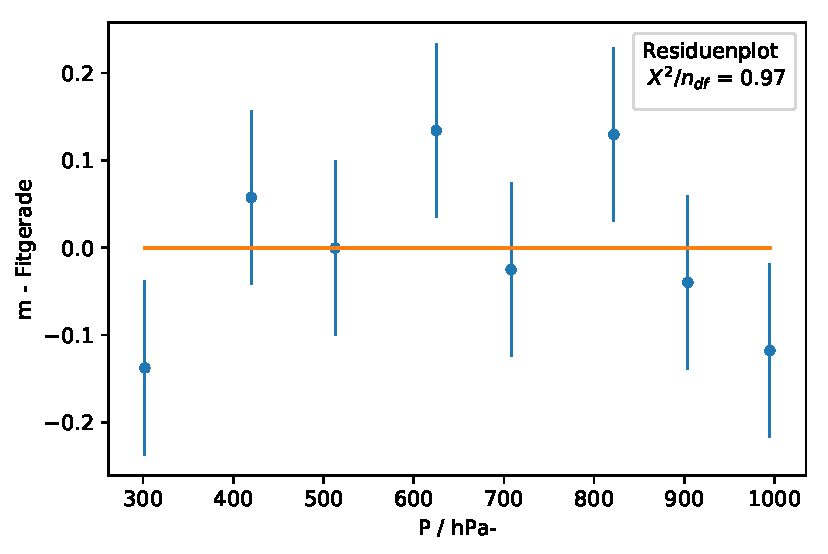
\includegraphics[width=\textwidth]{Python/MR7_Residuen.pdf}
	\end{subfigure}
	\caption{Lineare Regression mit der Messreihe 7}
	\label{MR7_LinReg}
\end{figure}


\end{document}